\documentclass[aspectratio=169,9pt]{beamer}
\graphicspath{{figures/}} % Setting the graphicspath

% Theme settings
\usetheme{Madrid}
\usecolortheme{default}
\setbeamertemplate{navigation symbols}{}   % removes navigation symbols such as 'next page'
\setbeamertemplate{footline}{}             % remove line with name, date, page nr. 
\setbeamercolor*{frametitle}{bg=white}     % remove background from frametitle
\usepackage{caption}
% \captionsetup[figure]{labelformat=empty}% redefines the caption setup of the figures environment in the beamer class.
\setbeamersize{text margin left=20pt,text margin right=10pt}

\usefonttheme[onlymath]{serif} % makes beamer math look like article math


%======================= import packages =======================
\usepackage{pifont}       % Pi fonts (Digbats, symbol, etc.)
\usepackage{graphicx}     % More options for \includegraphics
\usepackage{tikz}
\usepackage{appendixnumberbeamer} % separate appendix numbering
\usepackage{booktabs}
\usepackage{hyperref}
\usepackage{tabularx}
\usepackage{amsmath, nccmath}


%======================= page numbering =======================
\addtobeamertemplate{navigation symbols}{}{ \usebeamerfont{footline}
  \insertframenumber / \inserttotalframenumber \hspace*{2mm} \\ \vspace*{1mm} 
}


%=================================== colors ===================================
\definecolor{RoyBlue}{RGB}{22, 46, 69}
\definecolor{RoyGrey}{RGB}{64, 88, 128} 

\newcommand{\hlme}[1]{{\color{red}\bf #1}} % highlight me

\setbeamercolor{structure}{fg=RoyBlue} % itemize, enumerate, etc
\setbeamercolor{frametitle}{fg=RoyGrey}
 \setbeamercolor{section in head/foot}{bg=RoyBlue}


%======================= add progress dots to headline =======================
\setbeamertemplate{headline}{%
    \begin{beamercolorbox}[ht=4mm,dp=4mm]{section in head/foot}
        \insertnavigation{\paperwidth}
    \end{beamercolorbox}%
}%
\makeatother


%======================= add section title page =======================
\AtBeginSection[]{
  \begin{frame}
  \vfill
  \centering
    \usebeamerfont{title}\insertsection\par%
  \vfill
  \end{frame}
}


% \AtBeginSection[]{
%   \begin{frame}
%   %\vfill
%   \centering
%   \begin{beamercolorbox}[sep=8pt,center,shadow=true,rounded=true]{testttt}
%     \usebeamerfont{asdfasdfa}\insertsection\par%
%   \end{beamercolorbox}
%   %\vfill
%   \end{frame}
% }



%=================================== titlepage ===================================
\title{The NNPDF4.0 global analysis of the proton structure}
\date{DIS 2022, 3 May 2022}
\author{Roy Stegeman}
\institute{University of Milan and INFN Milan}
\titlegraphic{\vspace*{6mm}
    
\includegraphics[height=0.8cm]{logos/LOGO-ERC.jpg} \hspace{10mm}
	
\includegraphics[height=0.8cm]{logos/n3pdflogo_noback.png} \hspace{10mm}
	
\includegraphics[height=0.6cm]{logos/nnpdf_logo_official.pdf} \hspace{10mm}
	\includegraphics[height=0.8cm]{logos/Logo_Università_degli_Studi_di_Milano(not_mandatory).png}
	
\includegraphics[height=0.8cm]{logos/INFN_logo.png}
    \vspace*{5mm} \\
	\centering{ 
	\fontsize{7.0pt}{0.0pt}\selectfont This project has received funding from the European Union’s Horizon 2020 \\	
    \vspace*{-1mm}
	research and innovation programme under grant agreement No 740006.
	}
}

\defbeamertemplate{title page}{noinstitute}[1][]
{
  \vbox{}
  \vfill
  \begingroup
    \centering
    \begin{beamercolorbox}[sep=8pt,center,#1]{title}
      \usebeamerfont{title}\inserttitle\par%
      \ifx\insertsubtitle\@empty%
      \else%
        \vskip0.25em%
        {\usebeamerfont{subtitle}\usebeamercolor[fg]{subtitle}\insertsubtitle\par}%
      \fi%     
    \end{beamercolorbox}%
    \vskip1em\par
    \begin{beamercolorbox}[sep=0pt,center,#1]{author}
      \usebeamerfont{author}\insertauthor
    \end{beamercolorbox}
	\begin{beamercolorbox}[sep=0pt,center,#1]{author}
		\usebeamerfont{institute}\insertinstitute
	\end{beamercolorbox}
	\vspace*{8pt}
	\begin{beamercolorbox}[sep=0pt,center,#1]{author}
		On behalf of the NNPDF Collaboration \\
        {\small Based on: \href{https://arxiv.org/abs/2109.02653}{arXiv:2109.02653}}
	\end{beamercolorbox}
	\vspace*{16pt}
    \begin{beamercolorbox}[sep=0pt,center,#1]{date}
      \usebeamerfont{date}\insertdate
    \end{beamercolorbox}\vskip0.5em
    {\usebeamercolor[fg]{titlegraphic}\inserttitlegraphic\par}
  \endgroup
  \vfill
}

\makeatletter
\setbeamertemplate{title page}[noinstitute][colsep=-4bp,rounded=true,shadow=\beamer@themerounded@shadow]
\makeatother




\definecolor{Red}{rgb}{1,0,0}
\definecolor{Green}{rgb}{0,1,0}
\definecolor{Blue}{rgb}{0,0,1}
\definecolor{Gray}{gray}{0.9}
\definecolor{springgreen}   {cmyk}{0.26, 0   , 0.76, 0   }
\definecolor{olivegreen}    {cmyk}{0.64, 0   , 0.95, 0.40}
\definecolor{emerald}       {cmyk}{1   , 0   , 0.50, 0   }
\definecolor{junglegreen}   {cmyk}{0.99, 0   , 0.52, 0   }
\definecolor{seagreen}      {cmyk}{0.69, 0   , 0.50, 0   }
\definecolor{green}         {cmyk}{1   , 0   , 1   , 0   }
\definecolor{forestgreen}   {cmyk}{0.91, 0   , 0.88, 0.12}
\definecolor{pinegreen}     {cmyk}{0.92, 0   , 0.59, 0.25}
\definecolor{sepia}         {cmyk}{0   , 0.83, 1   , 0.70}
\definecolor{cerulean}      {cmyk}{0.94, 0.11, 0   , 0   }
\definecolor{salmon}        {cmyk}{0   , 0.53, 0.38, 0   }
\definecolor{greenyellow}   {cmyk}{0.15, 0   , 0.69, 0   }
\definecolor{arsenic}       {rgb}{0.23, 0.27, 0.29}
\definecolor{britishracinggreen}{rgb}{0.0, 0.26, 0.15}
\definecolor{oxfordblue}{rgb}{0.0, 0.13, 0.28}
\definecolor{bostonuniversityred}{rgb}{0.8, 0.0, 0.0}
\definecolor{goldenyellow}{rgb}{1.0, 0.87, 0.0}

\definecolor{darkgreen}{rgb}{0.0, 0.5, 0.13}
\definecolor{darkred}{rgb}{0.55, 0.0, 0.0}
\newcommand{\gct}{\color{darkgreen}\checkmark}
\newcommand{\rma}{\color{red}\ding{55}}
\newcommand{\bct}{\color{blue}\checkmark}
\newcommand{\arrowdownunder}{\begin{center}$\big\downarrow$\end{center}\vspace{-0.3cm}}
\newcommand{\mycolutitle}[1]{\vspace{-0.7cm}\begin{center}#1\end{center}\vspace{-0.1cm}}



\begin{document}
{
\setbeamertemplate{headline}{} % remove headline from titlepage
\begin{frame}
  \titlepage
\end{frame}
}




%======================= tikz settings =======================
\usetikzlibrary{shapes, arrows}
\usetikzlibrary{decorations.pathreplacing}
\usetikzlibrary{positioning, calc}
\tikzstyle{fitted} = [rectangle, minimum width=5cm, minimum height=1cm, text centered, draw=black, fill=red!30]
\tikzstyle{operations} = [rectangle, rounded corners, minimum width=2cm,text centered, draw=black, fill=red!30]
\tikzstyle{roundtext} = [rectangle, rounded corners, minimum width=2cm, minimum height=0.8cm, text centered, draw=black, fill=red!30]
\tikzstyle{n3py} = [rectangle, rounded corners, minimum width=3cm, minimum height=1cm, text centered, draw=black, fill=green!30]
\tikzstyle{myarrow} = [thick,->,>=stealth]
\tikzstyle{line} =[draw, -latex']
\tikzstyle{decision} = [diamond, draw, fill=red!20, text width=7.5em, text centered,  inner sep=0pt, minimum height=2em, aspect=4]
\tikzstyle{cloud} = [draw, ellipse,fill=green!20, minimum height=2em]
\tikzstyle{inout} = [rectangle, draw, fill=green!20, text width=9.5em, text centered, rounded corners, minimum height=2em, minimum width=10em]
\tikzstyle{block}=[rectangle, draw, fill=blue!20, text width=9.5em, 
                   text centered, rounded corners, minimum height=2em, 
                   minimum width=10em]
\tikzstyle{arrow} = [thick,->,>=stealth]

\pgfdeclarelayer{bg}    % declare background layer
\pgfsetlayers{bg,main}  % set the order of the layers (main is the standard layer)




% INTRO ========================================================================
\section*{NNPDF4.0}

\begin{frame}[t]{High-precision: gluon}
	\begin{equation*}
	\mathcal{L}_{i j}\left(M_{X}, y, \sqrt{s}\right)
	=\frac{1}{s} \sum_{i, j} f_{i}\left(\frac{M_{X} e^{y}}{\sqrt{s}}, M_{X}\right) f_{j}\left(\frac{M_{X} e^{-y}}{\sqrt{s}}, M_{X}\right)
	\end{equation*}
	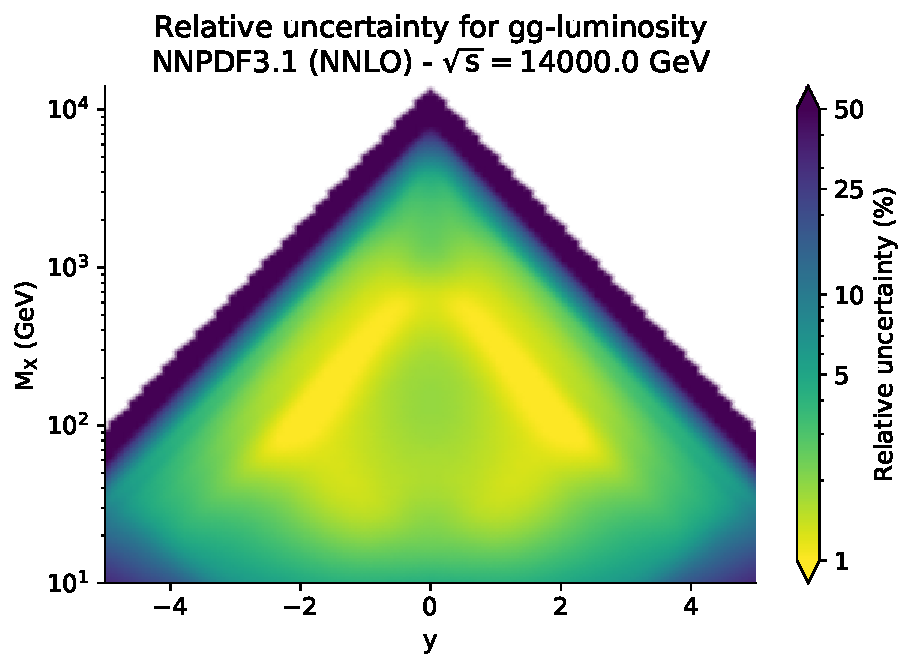
\includegraphics[width=0.45\textwidth]{plot_lumi2d_uncertainty_NNPDF31_gg}
	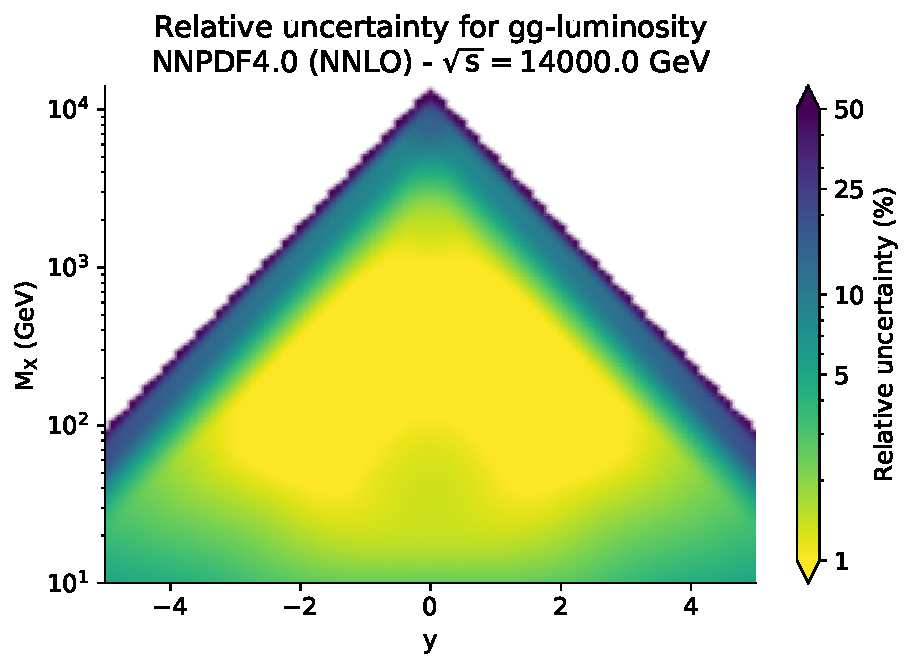
\includegraphics[width=0.45\textwidth]{plot_lumi2d_uncertainty_NNPDF40_gg}
    \begin{center}
	    \textbf{How did we get here?}
	\end{center}
\end{frame}

\begin{frame}[t]{High-precision: singlet }
	\begin{equation*}
	\mathcal{L}_{i j}\left(M_{X}, y, \sqrt{s}\right)
	=\frac{1}{s} \sum_{i, j} f_{i}\left(\frac{M_{X} e^{y}}{\sqrt{s}}, M_{X}\right) f_{j}\left(\frac{M_{X} e^{-y}}{\sqrt{s}}, M_{X}\right)
	\end{equation*}
	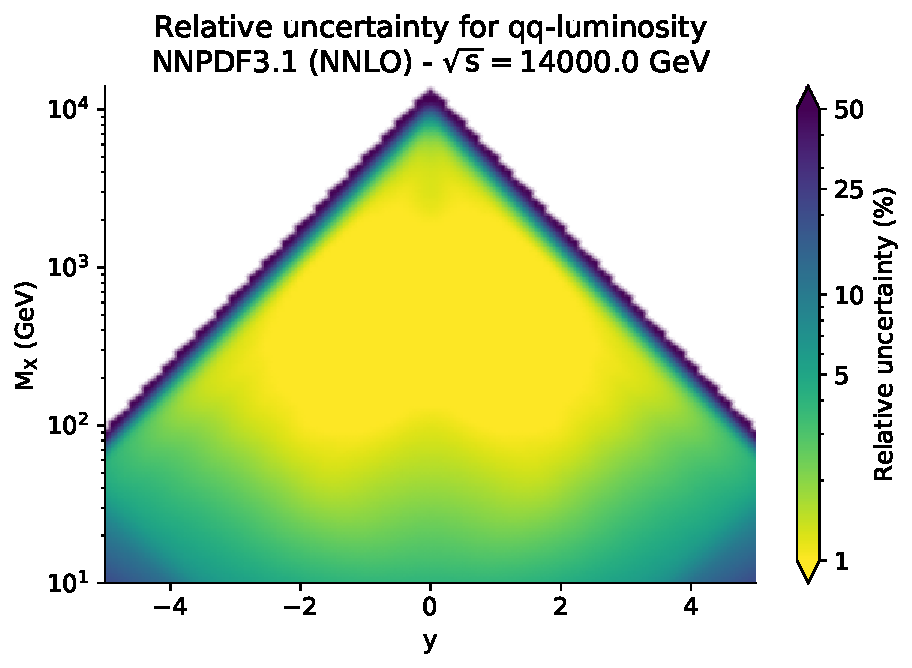
\includegraphics[width=0.45\textwidth]{plot_lumi2d_uncertainty_NNPDF31_qq}
	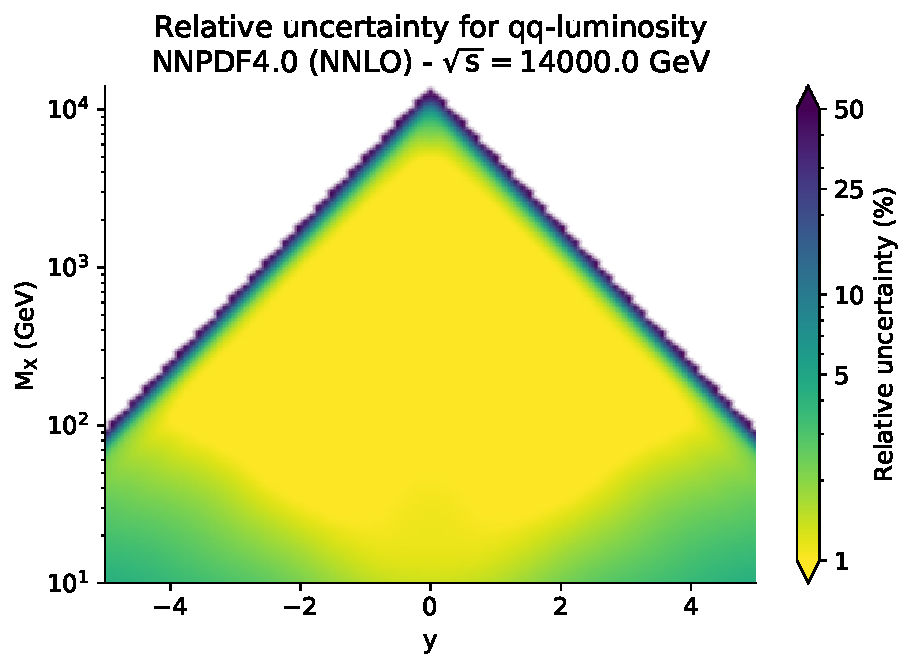
\includegraphics[width=0.45\textwidth]{plot_lumi2d_uncertainty_NNPDF40_qq}\\
	\begin{center}
	    \textbf{How did we get here?}
	\end{center}
\end{frame}






% DATA =========================================================================
\section{Data}

\begin{frame}{Data from NNPDF1.0 to NNPDF4.0}
	\begin{center}
		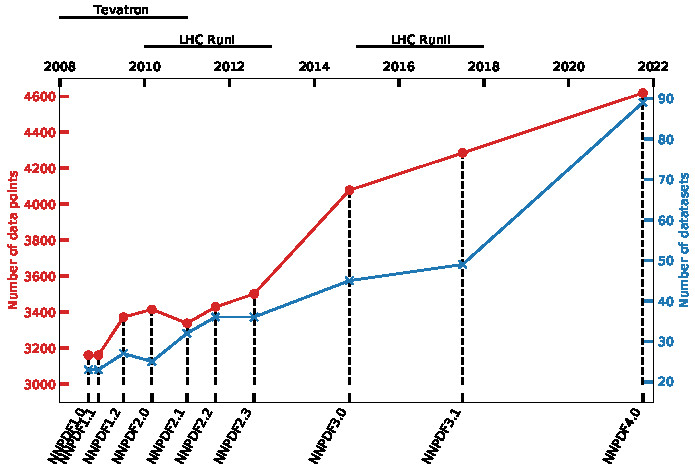
\includegraphics[width=0.5\textwidth]{NNPDF_data_history.pdf}
	\end{center}
	The number of datasets -- normally corresponding to different processes -- is generally more relevant than the number of datapoints
\end{frame}


\begin{frame}{Experimental data in NNPDF4.0}
    \begin{columns}
        \column{0.7\linewidth}
            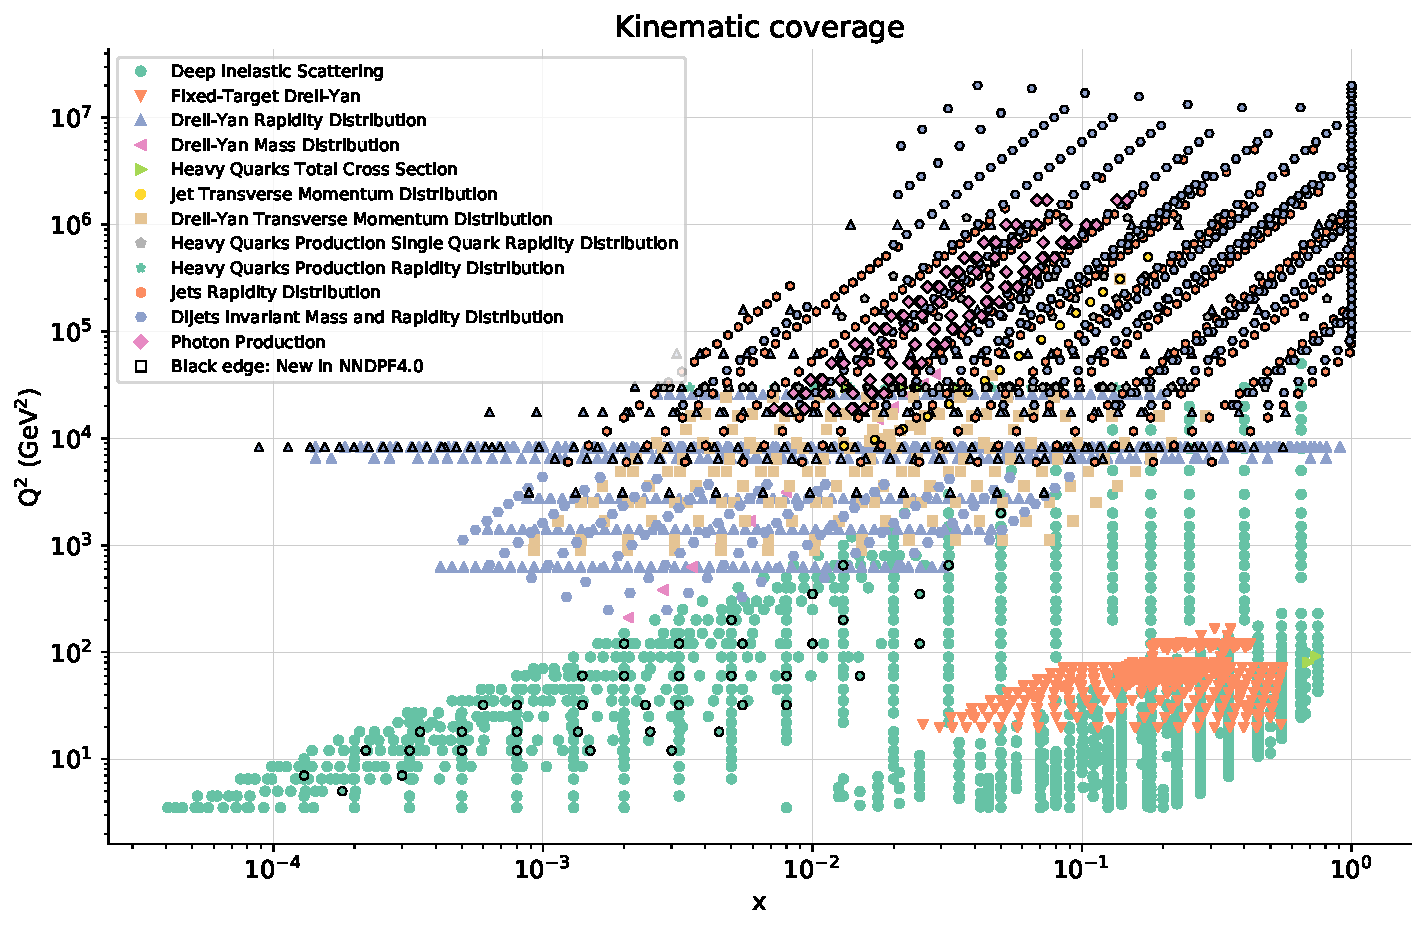
\includegraphics[width=1.0\textwidth]{Markers0_plot_xq2}
        \column{0.25\linewidth}
            New processes:
            \begin{itemize}
                \item direct photon
                \item single top
                \item dijets
                \item W+jet
                \item DIS jet
            \end{itemize}
    % \begin{block}{\footnotesize Theoretical improvement}
    % {\footnotesize
    % Nuclear uncertainties are included
    % }
    % \end{block}
    \end{columns}
\end{frame}








% METHODOLOGY ==================================================================
\section{Methodology}

\begin{frame}[t]{Improved fitting methodology}
    \begin{columns}[T]
        \begin{column}{0.48\textwidth}
            \begin{itemize}
                \item \textbf{Stochastic Gradient Descent} for NN training using TensorFlow
                \item Automated optimization of \\ \textbf{ model hyperparameters}
                \item Methodology is validated using 
                {\bf closure tests} (data region), {\bf future tests} (extrapolation region), and {\bf parametrization basis independence}
            \end{itemize}
        \vspace*{1em}
        Physical constraints:
        \begin{itemize}
            \item PDF positivity
            \item Integrability of nonsinglet distributions (Gottfried sum rules)
        \end{itemize}
        \end{column}
        \begin{column}{0.48\textwidth}
            \vspace*{-3em}
            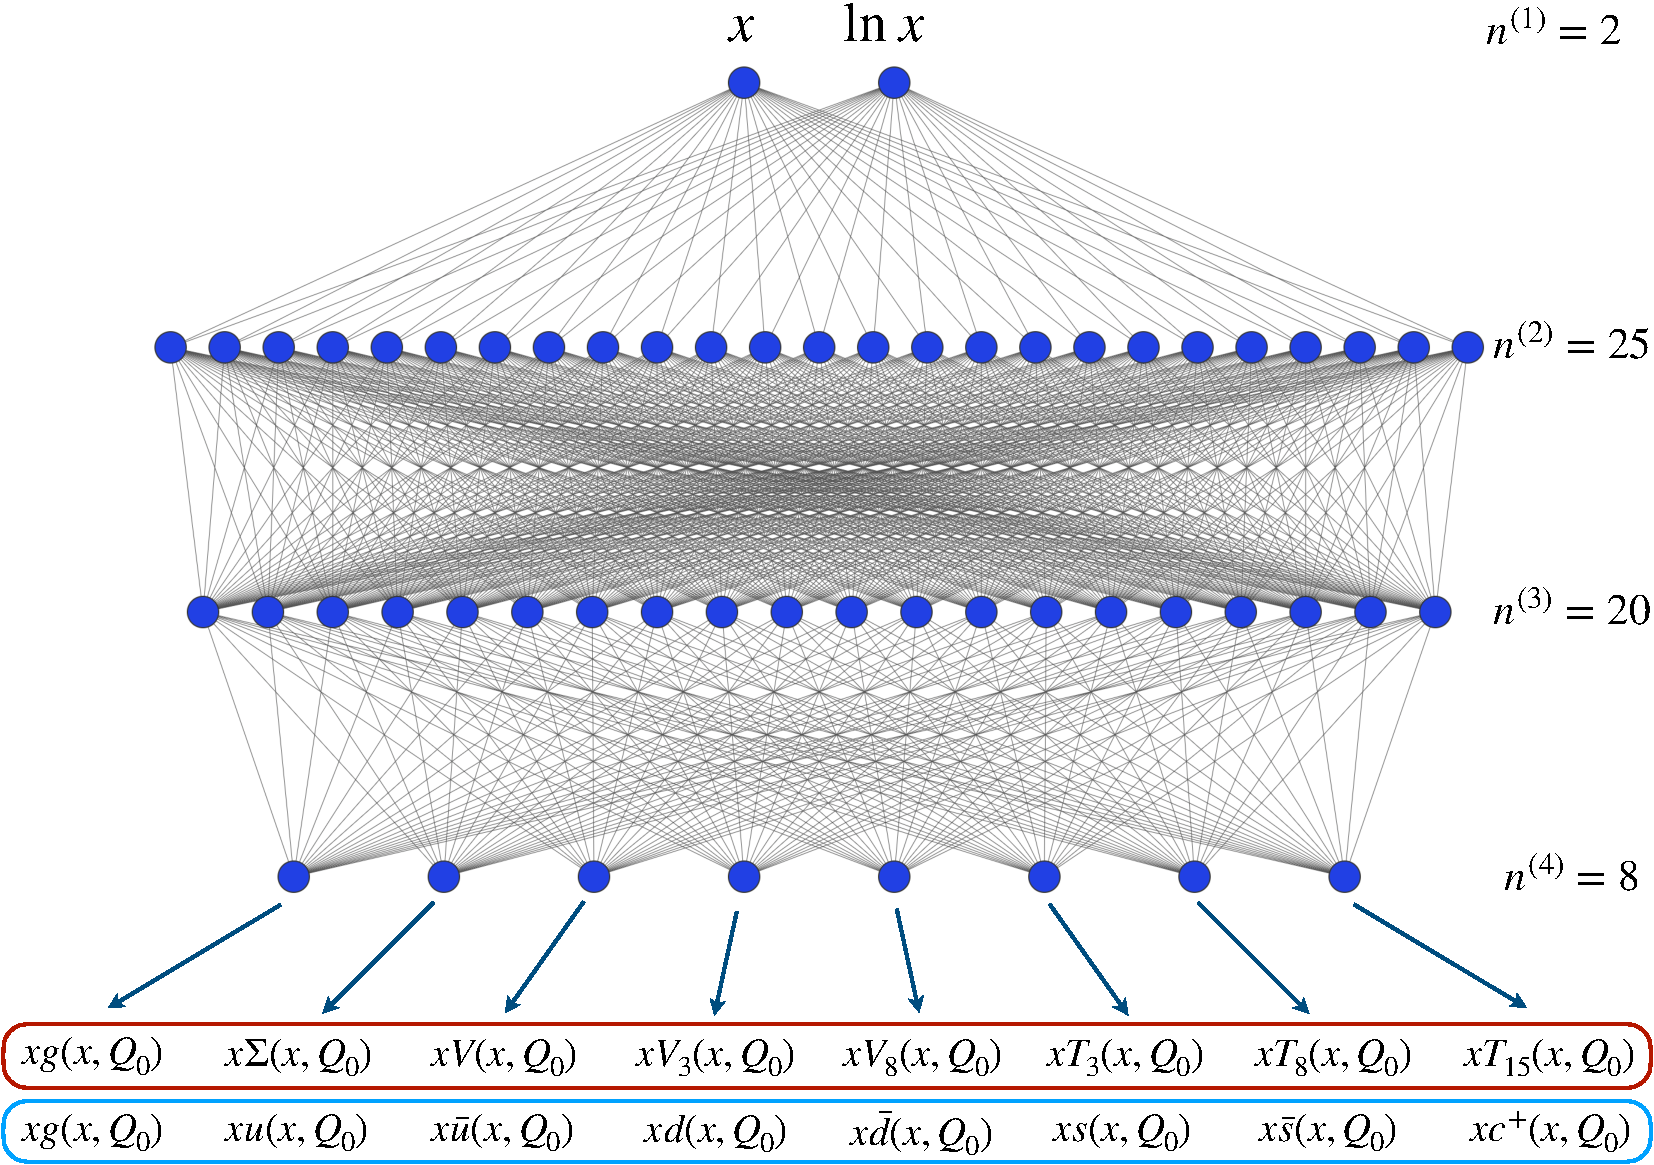
\includegraphics[width=1.0\textwidth]{NNarch}
            \begin{equation*}
                f_{i}\left(x, Q_{0}\right)=x^{-\alpha_{i}}(1-x)^{\beta_{i}} \mathrm{NN}_{i}(x)
            \end{equation*}
        \end{column}
    \end{columns}
\end{frame}


\begin{frame}[t]{Automated model selection}
	NNPDF aims to minimize sources of bias in the PDF:
	\begin{itemize}
	    \item Functional form $\rightarrow$ Neural Network
	    \item Model parameters $\rightarrow$ ?
	\end{itemize}
\end{frame}


\begin{frame}[t]{Automated model selection}
	NNPDF aims to minimize sources of bias in the PDF:
	\begin{itemize}
	    \item Functional form $\rightarrow$ Neural Network
	    \item Model parameters $\rightarrow$ \textbf{Hyperoptimization}
	\end{itemize}
    \begin{columns}
        \begin{column}{0.48\textwidth}
            Scan over thousands of hyperparameter combinations and select the best one \\
            \vspace*{0.8em}
            {\bf k-fold cross-validation}: used to define the reward function based on a {\bf test dataset}\\ 
            \vspace*{0.8em}
            Objective function: \\
            $L=\textrm{mean}(\chi_1^2,\chi_3^2,\chi_2^2,\ldots, \chi_k^2)$
        \end{column}
        \begin{column}{0.48\textwidth}
            \begin{center}
                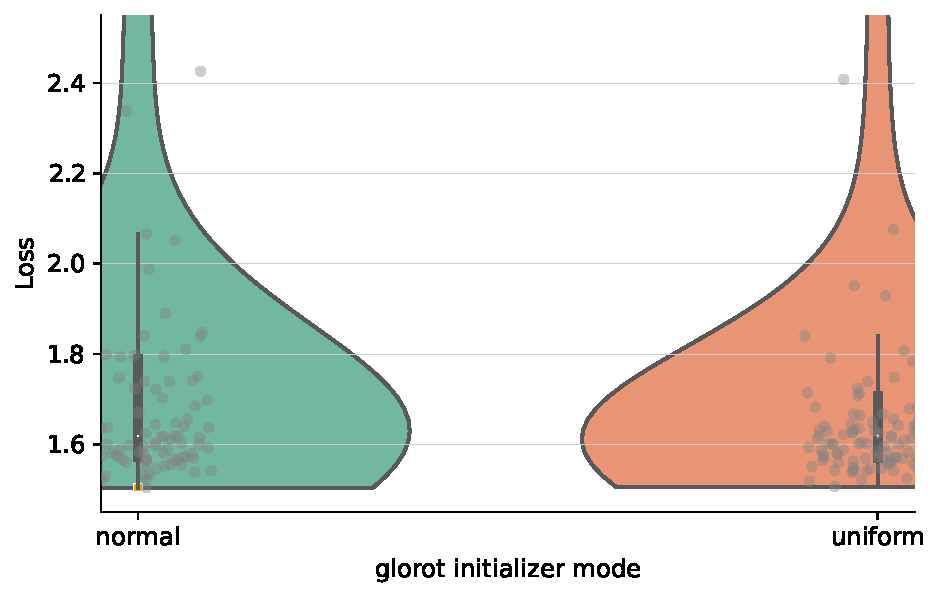
\includegraphics[width=0.48\textwidth]{sec_methodology_hyperopt_plot_initializer.pdf}
                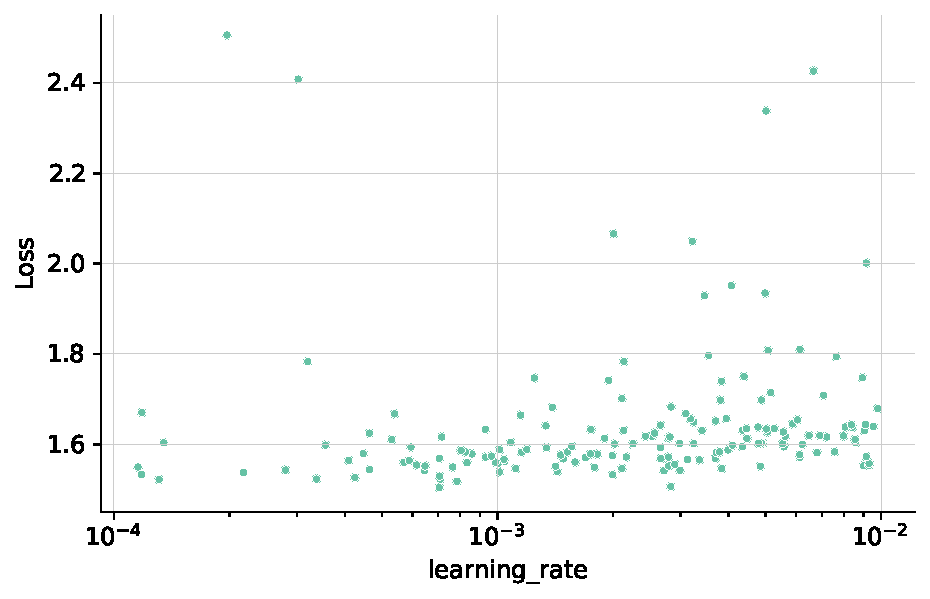
\includegraphics[width=0.48\textwidth]{sec_methodology_hyperopt_plot_lr.pdf} \\
                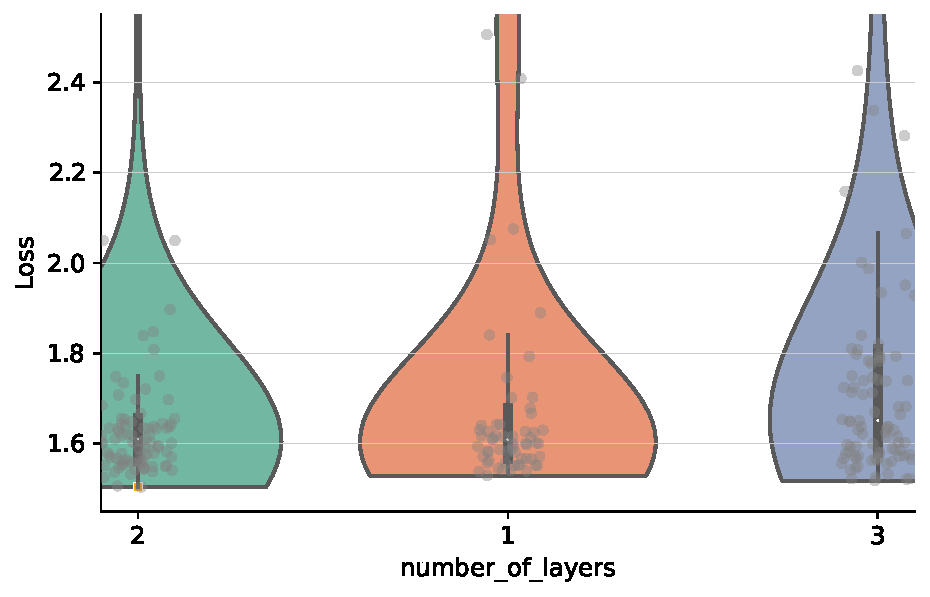
\includegraphics[width=0.48\textwidth]{sec_methodology_hyperopt_plot_number_of_layers.pdf}
                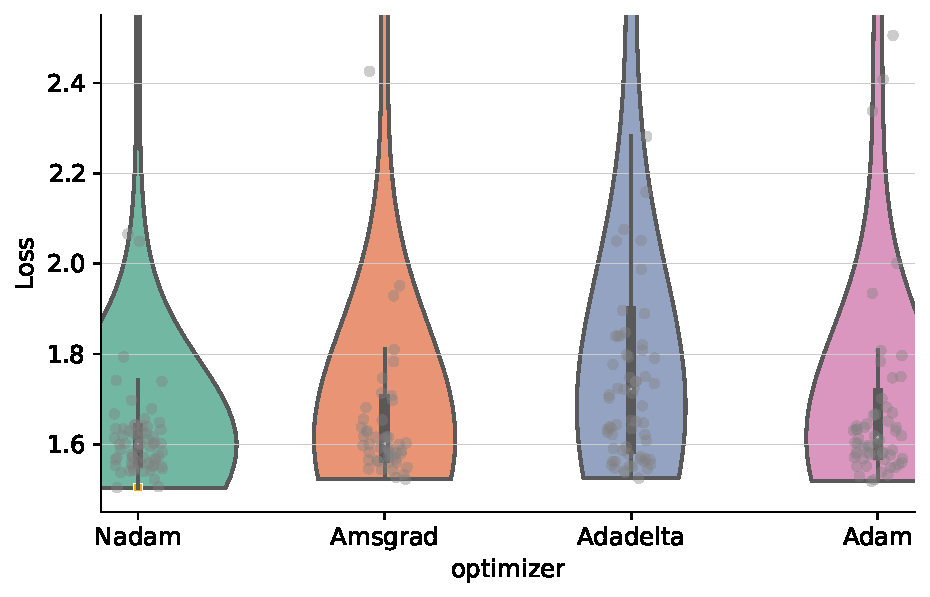
\includegraphics[width=0.48\textwidth]{sec_methodology_hyperopt_plot_optimizers.pdf}
            \end{center}
        \end{column}
    \end{columns}
\end{frame}





% Stability =======================================================
\section{Stability}
\begin{frame}{Parametrization basis independence}
    \begin{columns}
        \begin{column}[T]{0.48\textwidth}
        \vspace*{0pt}%
	        \begin{center}
	            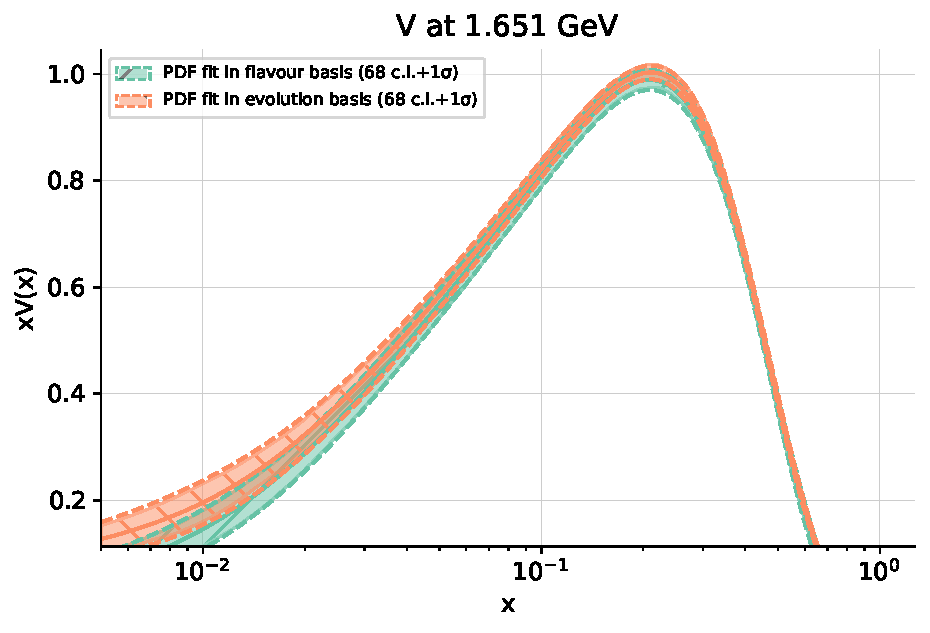
\includegraphics[width=0.8\textwidth]{flavour_evolution_V} \\
	        \end{center}
        \end{column}
        \begin{column}[t]{0.48\textwidth}
        \vspace{0pt}%
	        \begin{center}
	            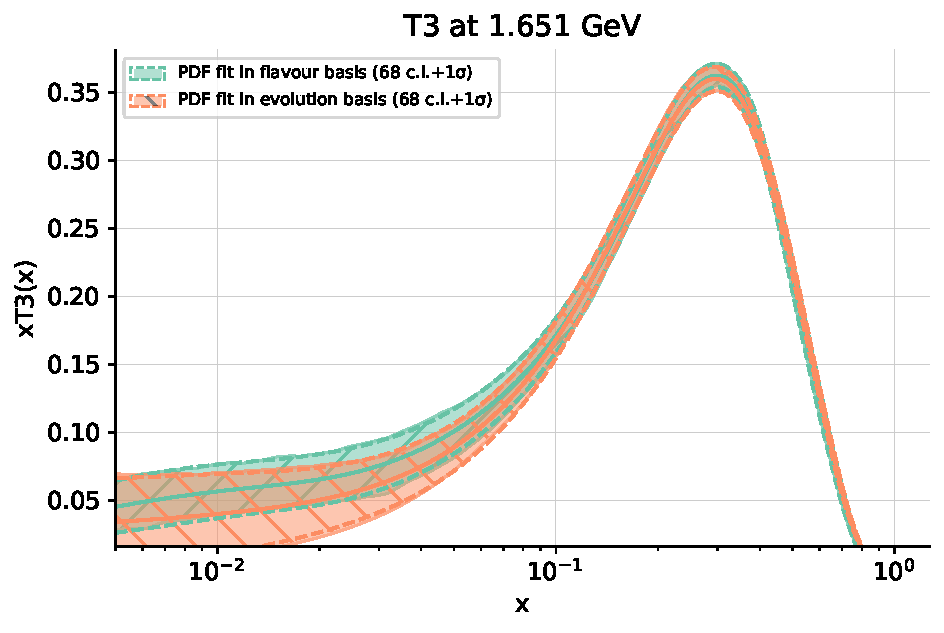
\includegraphics[width=0.8\textwidth]{flavour_evolution_T3} \\
	        \end{center}
        \end{column}
    \end{columns}
    \begin{columns}
        \column{0.4\linewidth}
		    Evolution Basis:
		    {\footnotesize
		    \begin{fleqn}
		    \begin{align*}
		       \qquad x V\left(x, Q_{0}\right) &\propto \mathrm{NN}_{V}(x)\\
		        x T_{3}\left(x, Q_{0}\right) &\propto \mathrm{NN}_{T_{3}}(x)
		    \end{align*}
		    \end{fleqn}
		    }
        \column{0.55\linewidth}
            \begin{block}{}
                Different strategies to parametrize the quark PDF flavour combinations leave the uncertainties essentially unchanged
            \end{block}
    \end{columns}
    \vspace*{-0.5em}
    Flavour Basis:
    {\footnotesize
    \begin{fleqn}
    \begin{align*}
        \qquad x V\left(x, Q_{0}\right) &\propto\left(\mathrm{NN}_{u}(x)-\mathrm{NN}_{\bar{u}}(x)+\mathrm{NN}_{d}(x)-\mathrm{NN}_{\bar{d}}(x)+\mathrm{NN}_{s}(x)-\mathrm{NN}_{\bar{s}}(x)\right) \\
        x T_{3}\left(x, Q_{0}\right) &\propto\left(\mathrm{NN}_{u}(x)+\mathrm{NN}_{\bar{u}}(x)-\mathrm{NN}_{d}(x)-\mathrm{NN}_{\bar{d}}(x)\right)
    \end{align*}
    \end{fleqn}
    }
\end{frame}

\begin{frame}[t]{Impact of the new data}
	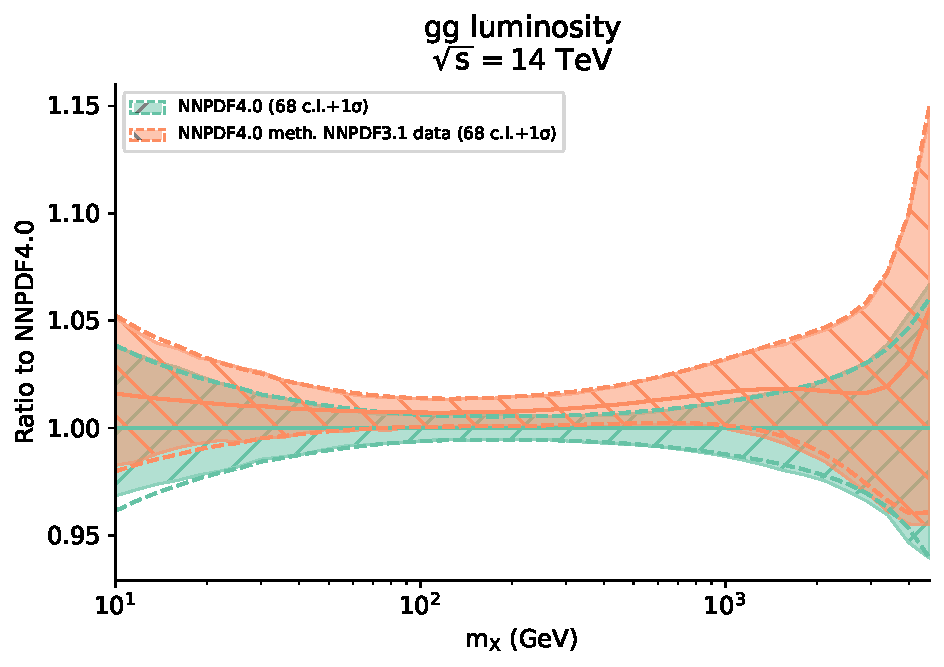
\includegraphics[width=0.45\textwidth]{lumi1d_gg_NNPDF40meth_NNPDF31data}
	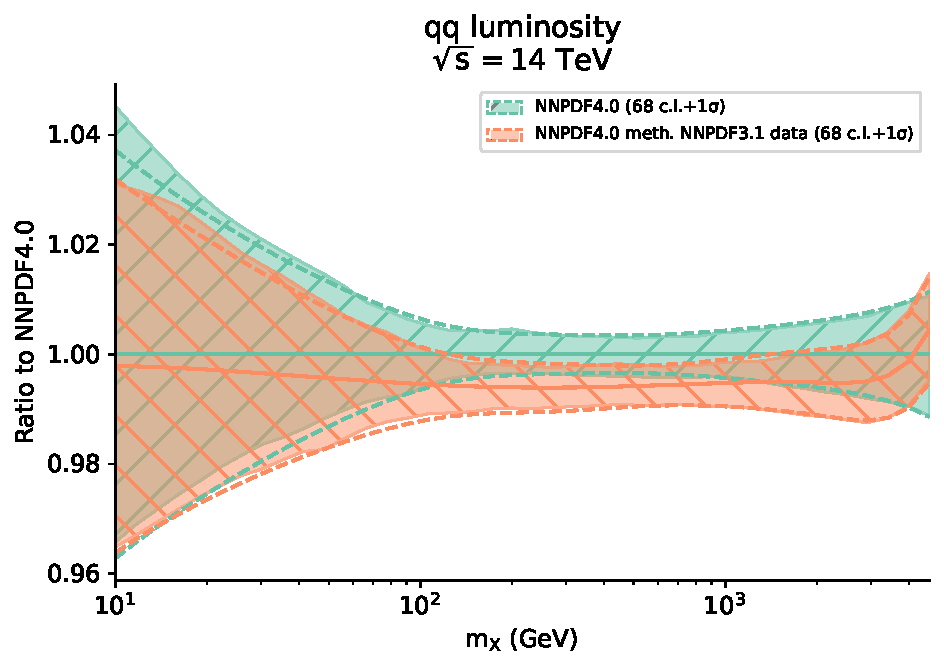
\includegraphics[width=0.45\textwidth]{lumi1d_qq_NNPDF40meth_NNPDF31data}
	Individual datasets have a limited impact, but collectively they result in:
	\begin{itemize}
	    \item Moderate reduction of PDF uncertainties
	    \item Shifts in central value at the one-sigma level
	\end{itemize}
\end{frame}


\begin{frame}[t]{Impact of the new fitting methodology}
	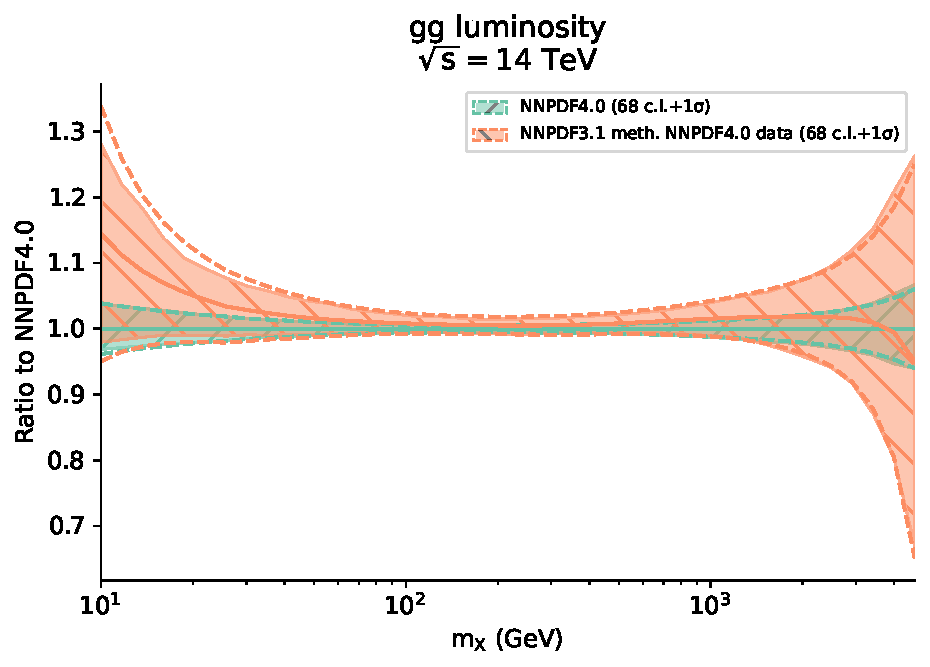
\includegraphics[width=0.45\textwidth]{lumi1d_gg_NNPDF31meth_NNPDF40data}
	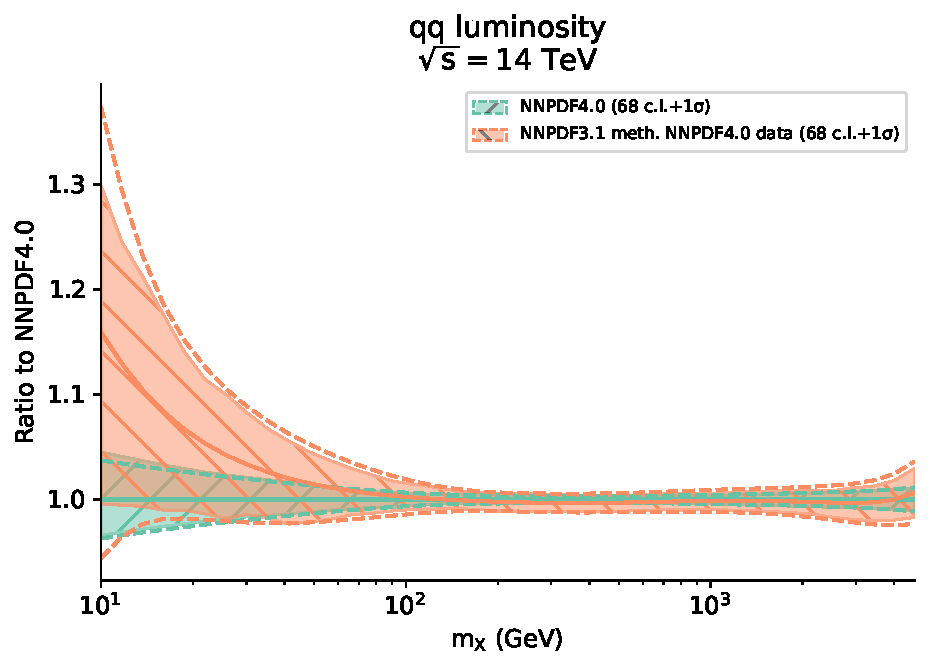
\includegraphics[width=0.45\textwidth]{lumi1d_qq_NNPDF31meth_NNPDF40data}
	\begin{columns}
	    \column{0.45\linewidth}
			\begin{itemize}
	    	        \item Significant reduction of PDF uncertainties
		        \item Good agreement between the central values
		    \end{itemize}
        \column{0.5\linewidth}
            \begin{block}{}
                \fontsize{7}{6}\selectfont
                PDF uncertainties are validated using closure tests and future tests\\
                Validation tests successful for both NNPDF4.0 and NNPDF3.1 
            \end{block}
    \end{columns}
\end{frame}



% PHENOMENOLOGY ================================================================
\section{LHC phenomenology}
\begin{frame}[t]{Implications for LHC phenomenology}
    \begin{center}
        Reduced luminosity uncertainties $\rightarrow$ Reduced uncertainty at the level of observables\\
        \vspace*{-0.5em}
        \begin{columns}
          \begin{column}{0.48\textwidth}
              \begin{center}
                  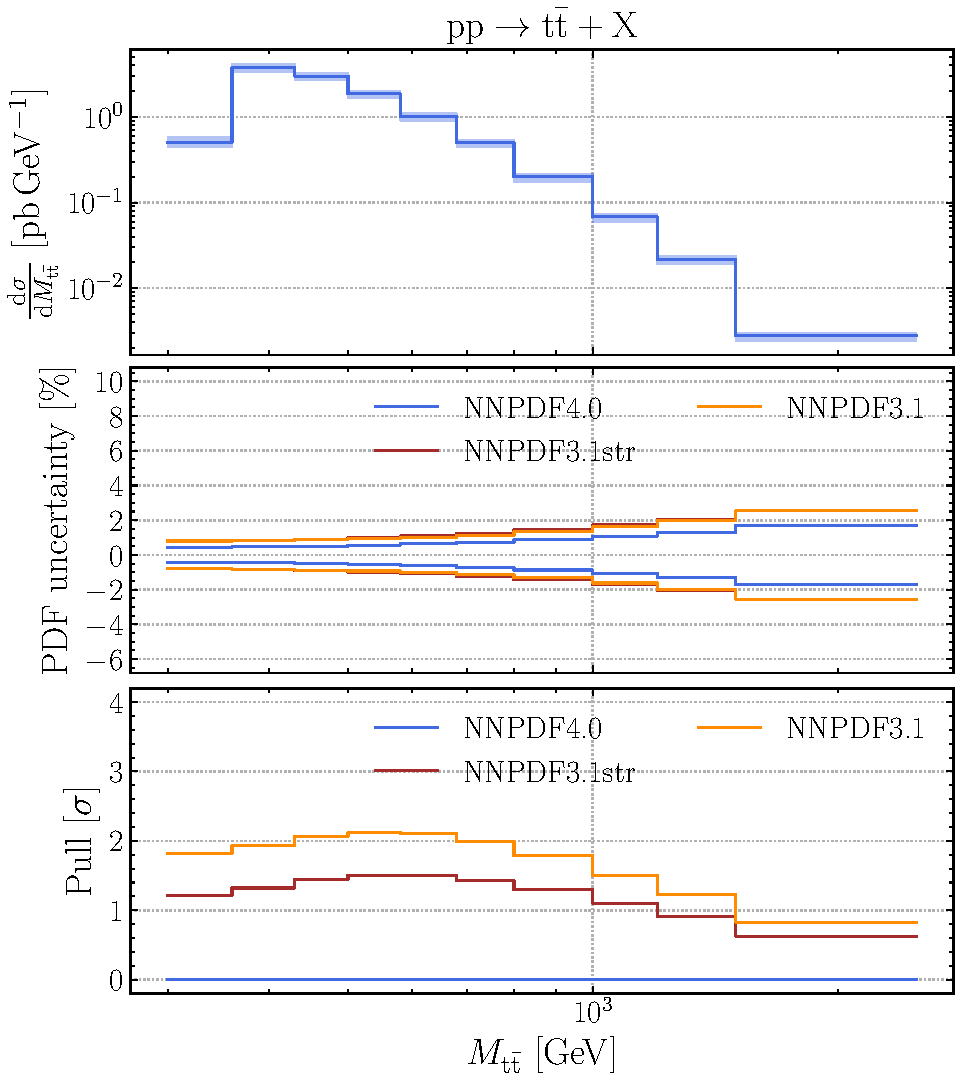
\includegraphics[width=0.78\textwidth]{NNPDF_TTB_14TEV_40_PHENO-internal} 
              \end{center}
          \end{column}
          \begin{column}{0.48\textwidth}
              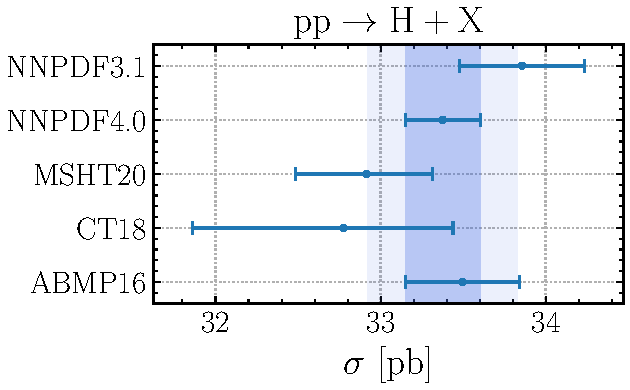
\includegraphics[width=0.7\textwidth]{NNPDF_H_14TEV_40_PHENO-integrated}\\
                  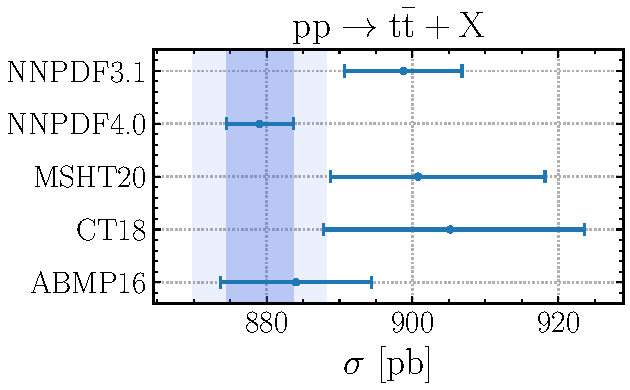
\includegraphics[width=0.7\textwidth]{NNPDF_TTB_14TEV_40_PHENO-integrated}
          \end{column}
        \end{columns}
    \end{center}
\end{frame}


% DELIVERY ====================================================================
\section{Open-source code}
\begin{frame}[t]{The open-source NNPDF code}
    The full NNPDF code has been made public along with user friendly documentation\\
    \vspace*{1em}
    This includes: fitting, hyperoptimization, theory, data processing, visualization\\
    \vspace*{1em}
    It is possible to reproduce all results of NNPDF4.0 and more!\\
    \vspace*{2em}
    \begin{block}{}
        \centering
		\href{https://link.springer.com/article/10.1140/epjc/s10052-021-09747-9}{Eur.Phys.J.C 81 (2021) 10, 958} \\
		\url{https://github.com/NNPDF/nnpdf} \\
		\url{https://docs.nnpdf.science}
    \end{block}
\end{frame}



% CONCLUSION ===================================================================
% \section{Beyond NNPDF4.0}

% \begin{frame}{Importance of scaling $x$}
%     \begin{center}
%         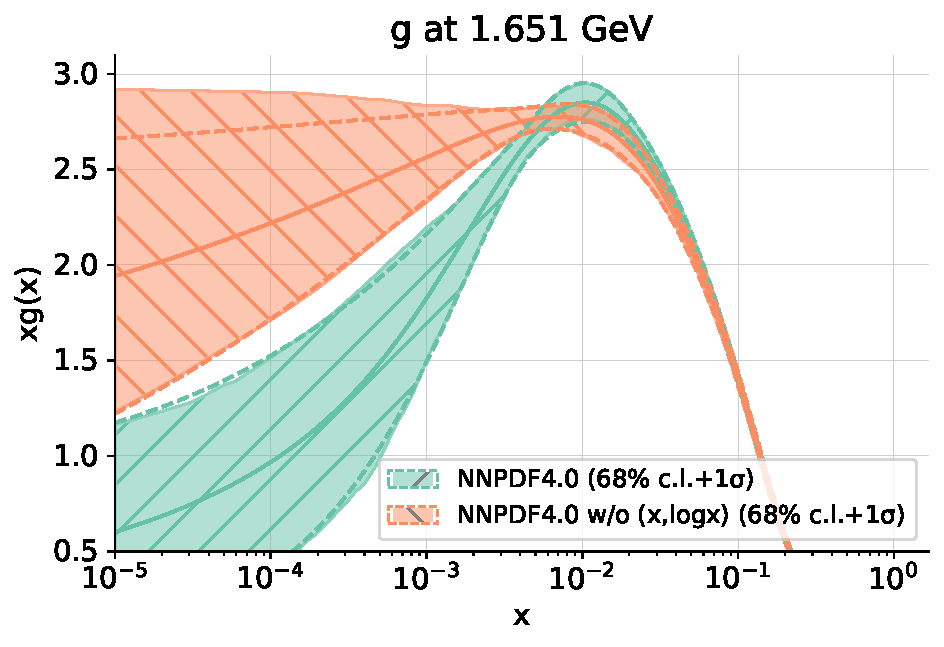
\includegraphics[width=0.45\textwidth]{pdf_g_without_xlogx.pdf}
%     \end{center}
%     \textbf{Problem:} Improper scaling of $x$ can lead to saturation of the neural network and affect the resulting PDFs, NNPDF solves this by passing ($x,\log x$) to the network \\
%     \vspace*{0.5em}
%     The convergence Gradient descent based algorithms struggles with inputs spanning different orders of magnitude
% \end{frame}


% \begin{frame}{Feature Scaling}{\href{https://link.springer.com/article/10.1140/epjc/s10052-022-10136-z}{\color{blue} Eur.Phys.J.C 82 (2022) 2}}
%     \textbf{Solution:} enforce all inputs $X$ to be on a similar scale \\
%     \textbf{How?} Map $X$ to grid of equidistant points using the emprical Cumulative Distribution Funciton (eCDF) \\
%     $ \hat{F}_n(x) = \frac{1}{n} \sum_{i=1}^{n} \mathbf{1}_{X_{i} \leq x}  $
%     \begin{center}
%         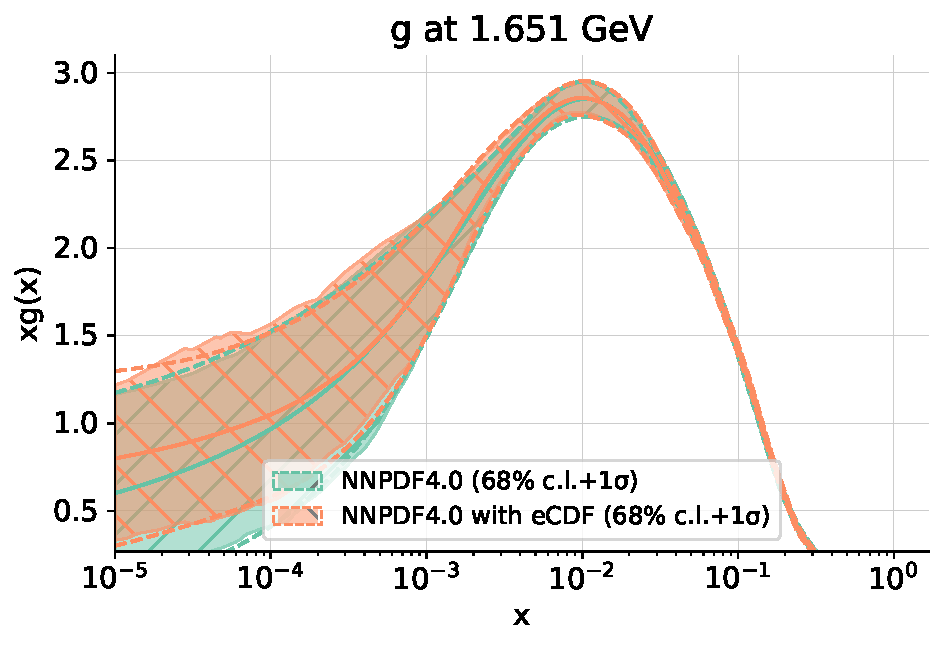
\includegraphics[width=0.45\textwidth]{pdf_gluon_log_ecdf_nnpdf40.pdf}
%     \end{center}
% \end{frame}


% \begin{frame}{Feature Scaling}{\href{https://link.springer.com/article/10.1140/epjc/s10052-022-10136-z}{\color{blue} Eur.Phys.J.C 82 (2022) 2}}
%     Convergence without preprocessing \\
%     \vspace*{0.5em}
%     $
%     f_{i}\left(x, Q_{0}\right)=x^{-\alpha_{i}}(1-x)^{\beta_{i}} \mathrm{NN}_{i}(x,\log x) 
%     \rightarrow
%     f_{i}\left(x, Q_{0}\right)= \mathrm{NN}_{i}(\hat{F}_n(x)) 
%     $\\
%     \vspace*{0.5em}
%     Saturation in the small-$x$ extrapolation region
%     \begin{center}
%         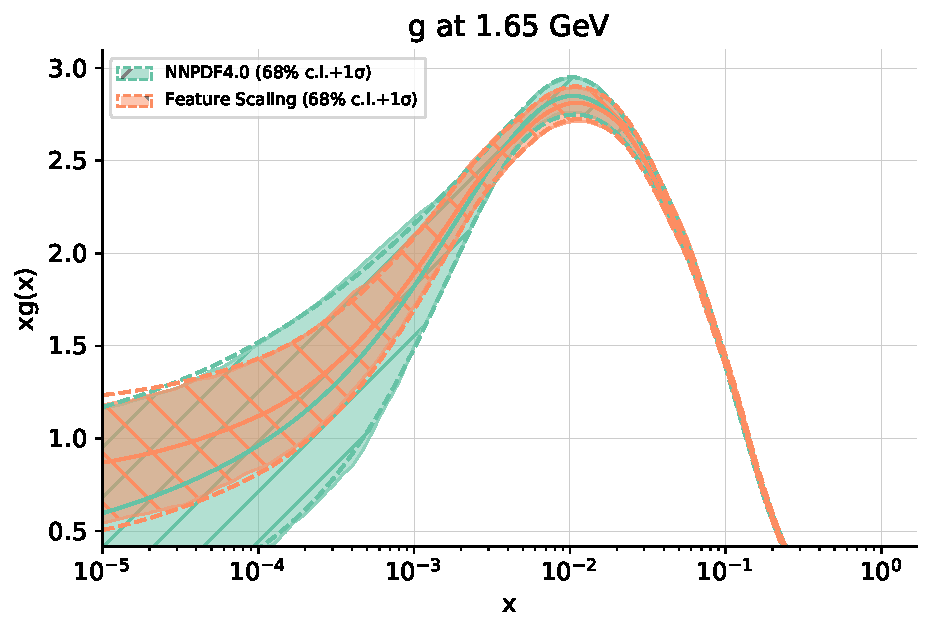
\includegraphics[width=0.45\textwidth]{pdf_gluon_log_feature_vs_nnpdf40.pdf}
%     \end{center}
% \end{frame}



% \begin{frame}[t]{Beyond $k$-folds hyperoptimization}

%     Statistical effects can screen out overfitting during hyperoptimization:

%     \begin{center}
%       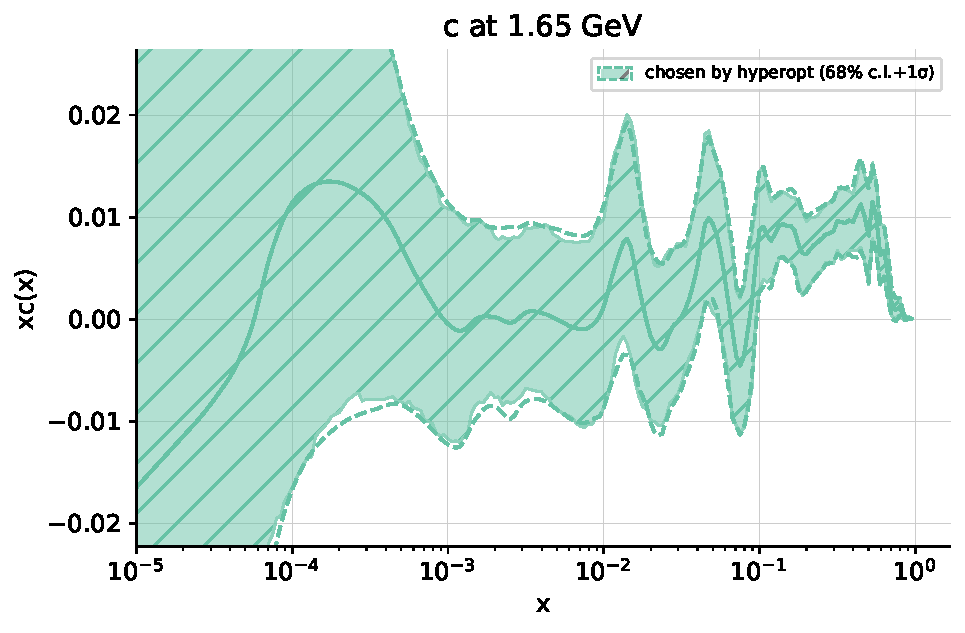
\includegraphics[width=0.4\textwidth]{hyperopt_choice_charm_plot_pdfs_c.pdf}
%       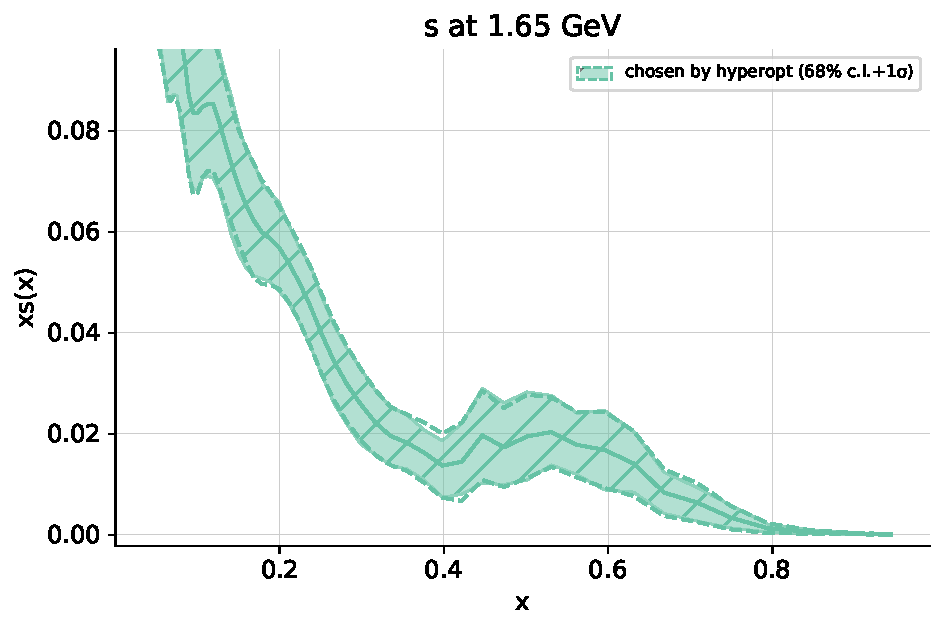
\includegraphics[width=0.4\textwidth]{hyperopt_choice_strange_plot_pdfs_s.pdf}
%     \end{center}
%     \begin{center}
%         \textbf{Can we quantify overfitting?}
%     \end{center}
% \end{frame}


% \begin{frame}[t]{A measure for overfitting}

%     \textbf{Idea:} for any PDF the validation loss to the fitted pseudodata $\chi^{r}_\text{val}$ should be equal to the loss calculated for any other pseudodata set  $\chi^{\hat{r}}_\text{val}$
%     \\\vspace*{1em}

%     Thus a metric for overfitting is
%     $$
%     \Delta\chi^2_{\text{overfit}}=\langle \chi^{2}_\text{val,$\hat{r}$} - \chi^{2}_\text {val,r}\rangle\quad (<0 \text{ if overfitted})
%     $$

%     % While \textbf{underfitted} setups will be filtered due to their higher $\chi^2$ values 

%     \begin{columns}
%         \begin{column}{0.48\textwidth}
%             \centering
%             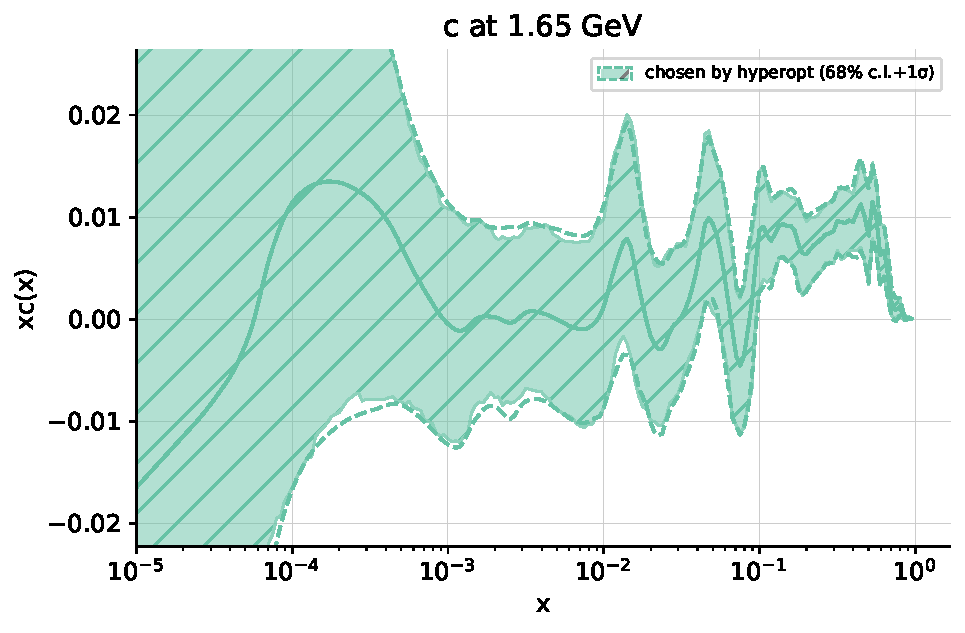
\includegraphics[width=0.8\textwidth]{hyperopt_choice_charm_plot_pdfs_c.pdf}
%             $\Delta\chi^2_{\text{overfit}}=-0.0459 \pm 0.0078$ \\
%             $5.9\sigma$ from 0
%         \end{column}
%         \begin{column}{0.48\textwidth}
%             \centering
%             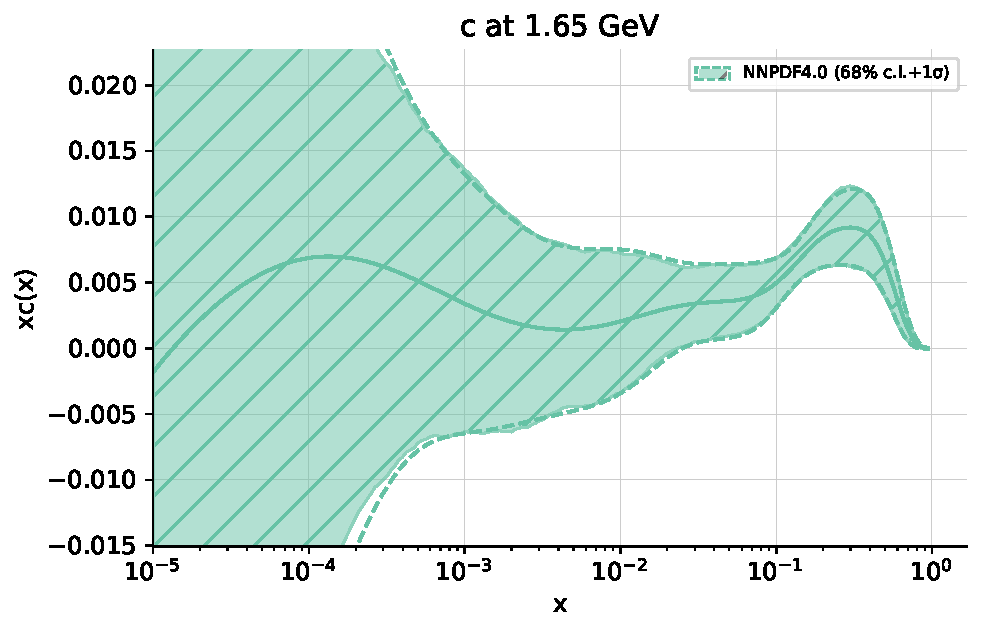
\includegraphics[width=0.8\textwidth]{NNPDF40_fit_charm_plot_pdfs_c.pdf}\\ 
%             $\Delta\chi^2_{\text{overfit}}=-0.0012 \pm 0.0130$ \\
%             $0.1\sigma$ from 0
%         \end{column}
%     \end{columns}


% \end{frame}


% CONCLUSION ===================================================================
\section{Summary and Outlook}
\begin{frame}[t]{Summary and Outlook}
    \begin{itemize}
        \item NNPDF4.0 is the latest release in the NNPDF family of PDF sets
        \item 44 new datasets from many new processes are included
        \item Improved methodology with Stochastic Gradient Descent and hyperoptimization
        \item Validation of PDF uncertainties using closure test, future test and parametrization basis independence
        \item[$\Rightarrow$] NNPDF4.0 achieves a high precision over a broad kinematic range
    \end{itemize}
	\vspace*{1em}
    \begin{itemize}
        \item The current level of PDF uncertainties challenges the accuracy of theoretical predictions and demands an increased effort towards the systematic inclusion in the fit of theoretical uncertainties (nuclear, higher orders, SM parameters, \ldots ) and higher-order QCD and EW corrections
    \end{itemize}


    \vspace*{1em}
    \only<2>{
    \begin{center}
        {\Large \textbf{Thank you!}}
    \end{center}
    }
\end{frame}




\begin{frame}{Determination of the photon PDF}
  \begin{columns}[T]
    \begin{column}{0.59\textwidth}
      Initially the photon PDF has been determined in different ways:
      \begin{itemize}
        \item physical model: sensitive to underlying model
        \item fitting: data does not provide strong constraints
      \end{itemize}

      \vspace*{0.5em}
      However with the LUXqed approach it can be computed perturbatively \\
      based on the observation that the heavy-lepton production cross-section can be written in two ways:
      \begin{itemize}
        \item in terms of structure functions $F_2$, $F_L$
        \item in terms of PDFs (including the photon)
      \end{itemize}

      \vspace*{0.5em}
      luxQED result {\color{gray}\small[Manohar, Nason, Salam, Zanderighi: 1607.04266, 1708.01256]}:
      \vspace*{-0.8em}
      \begin{equation*}
        \begin{split}
          & x \gamma(x, \mu^2)
          =
          \frac{2}{\alpha (\mu^2)} \int\limits_x^1 \frac{dz}{z}
          \Biggl\{ \int_{m_p^2x^2 \over 1-z}^{\mu^2 \over 1-z} \frac{dQ^2}{Q^2}
          \alpha^2(Q^2) \Biggl[ -z^2 F_L(x/z, Q^2) \\
          & + \left( z P_{\gamma q}(z) + \frac{2 x^2 m_p^2}{Q^2} \right)
          F_2(x/z, Q^2)\Biggr] - \alpha^2(\mu^2) z^2 F_2(x/z, \mu^2)\Biggr\}
        \end{split}
      \end{equation*}
    \end{column}

    \begin{column}{0.39\textwidth}
      \vspace*{-2.5em}
      \begin{figure}
        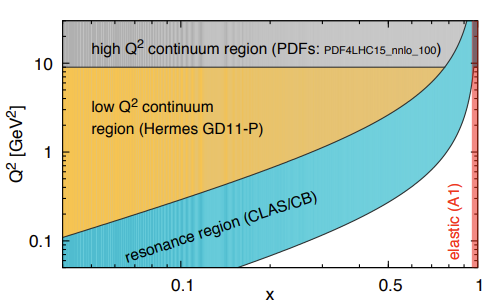
\includegraphics[width=0.89\textwidth]{figures/dataluxqed.png}
        \caption*{Input to construct $F_2$ and $F_L$}
        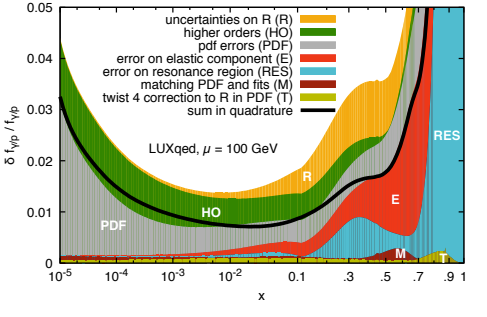
\includegraphics[width=0.89\textwidth]{figures/luxQED_uncs.png}
        \caption*{Sources of uncertainty}
      \end{figure}
    \end{column}
  \end{columns}
\end{frame}


\begin{frame}{LUXqed PDF determinations}
  LUXqed has been used in all of the most recent QED PDFs:
  \begin{itemize}
      \item LUXqed\_plus\_PDF4LHC15 {\color{gray}\small [1607.04266]}
      \item LUXqed17\_plus\_PDF4LHC15 {\color{gray}\small [1708.01256]}
      \item MMHT2015qed {\color{gray}\small [1907.02750]}
      \item NNPDF3.1luxQED {\color{gray}\small [1712.07053]}
      \item CT18lux and CT18qed {\color{gray}\small [2106.10299]}
      \item MSHT20QED {\color{gray}\small [2111.05357]}
      \item MSHT20qed\_an3lo {\color{gray}\small [2312.07665]}
      \item NNPDF4.0QED {\color{gray}\small [2401.08749 ]}
  \end{itemize}
\end{frame}

% \begin{frame}{Results: photon PDF and luminosity}
%   \begin{center}
%     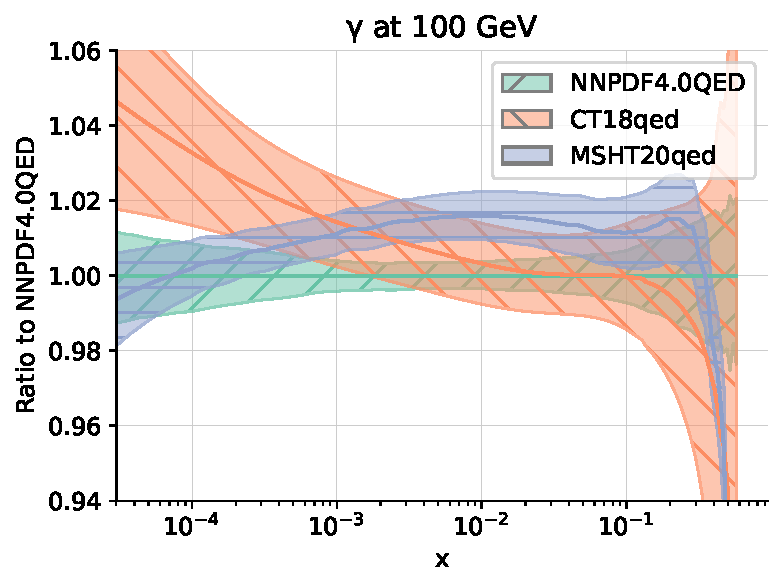
\includegraphics[width=0.3\textwidth]{figures/photon_comparison.pdf}
%     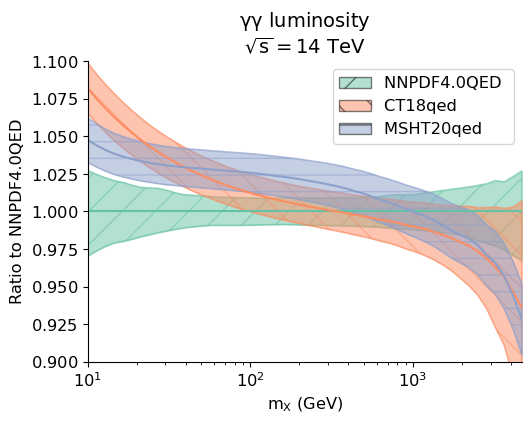
\includegraphics[width=0.3\textwidth]{figures/pp_lumi_comparison.png}
%     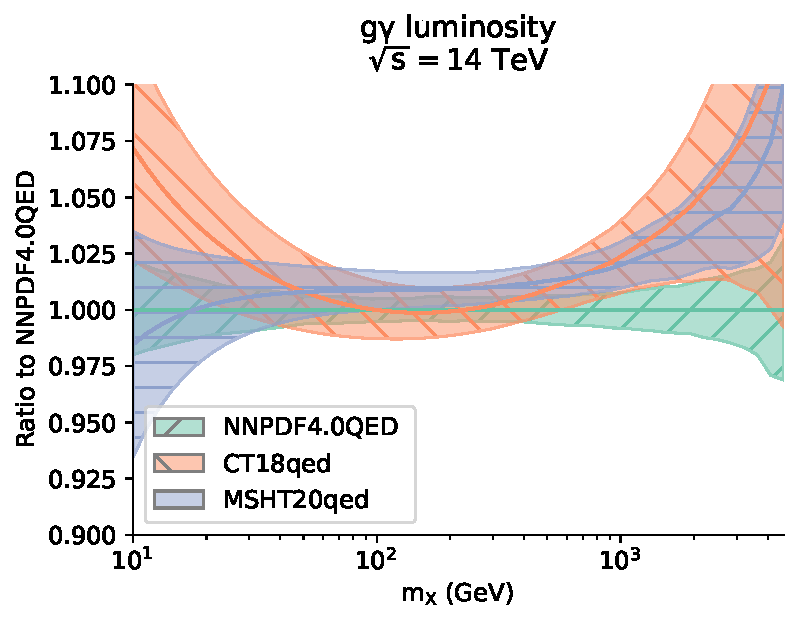
\includegraphics[width=0.3\textwidth]{figures/gp_lumi_comparison.pdf}
%   \end{center}
%   \begin{itemize}
%     \item Because all groups use the luxQED formalism, the photon PDFs agree at percent level
%     \item Luminosity generally in agreement, but differ at very small and very large invariant mass
%   \end{itemize}
% \end{frame}


% ============================================================================


\begin{frame}{Incomplete higher order uncertainties covmat}
  \begin{itemize}
    \item We construct an IHOU matrix following a similar approach by varying the subleading functions
    \item IHOU are independent of MHOU so the uncertainties are added in quadrature
    $$C = C_\mathrm{exp}+C_\mathrm{MHOU}+C_\mathrm{IHOU}$$
  \end{itemize}

  \begin{columns}
    \begin{column}{0.49\textwidth}
      \begin{figure}[!t]
        \centering
        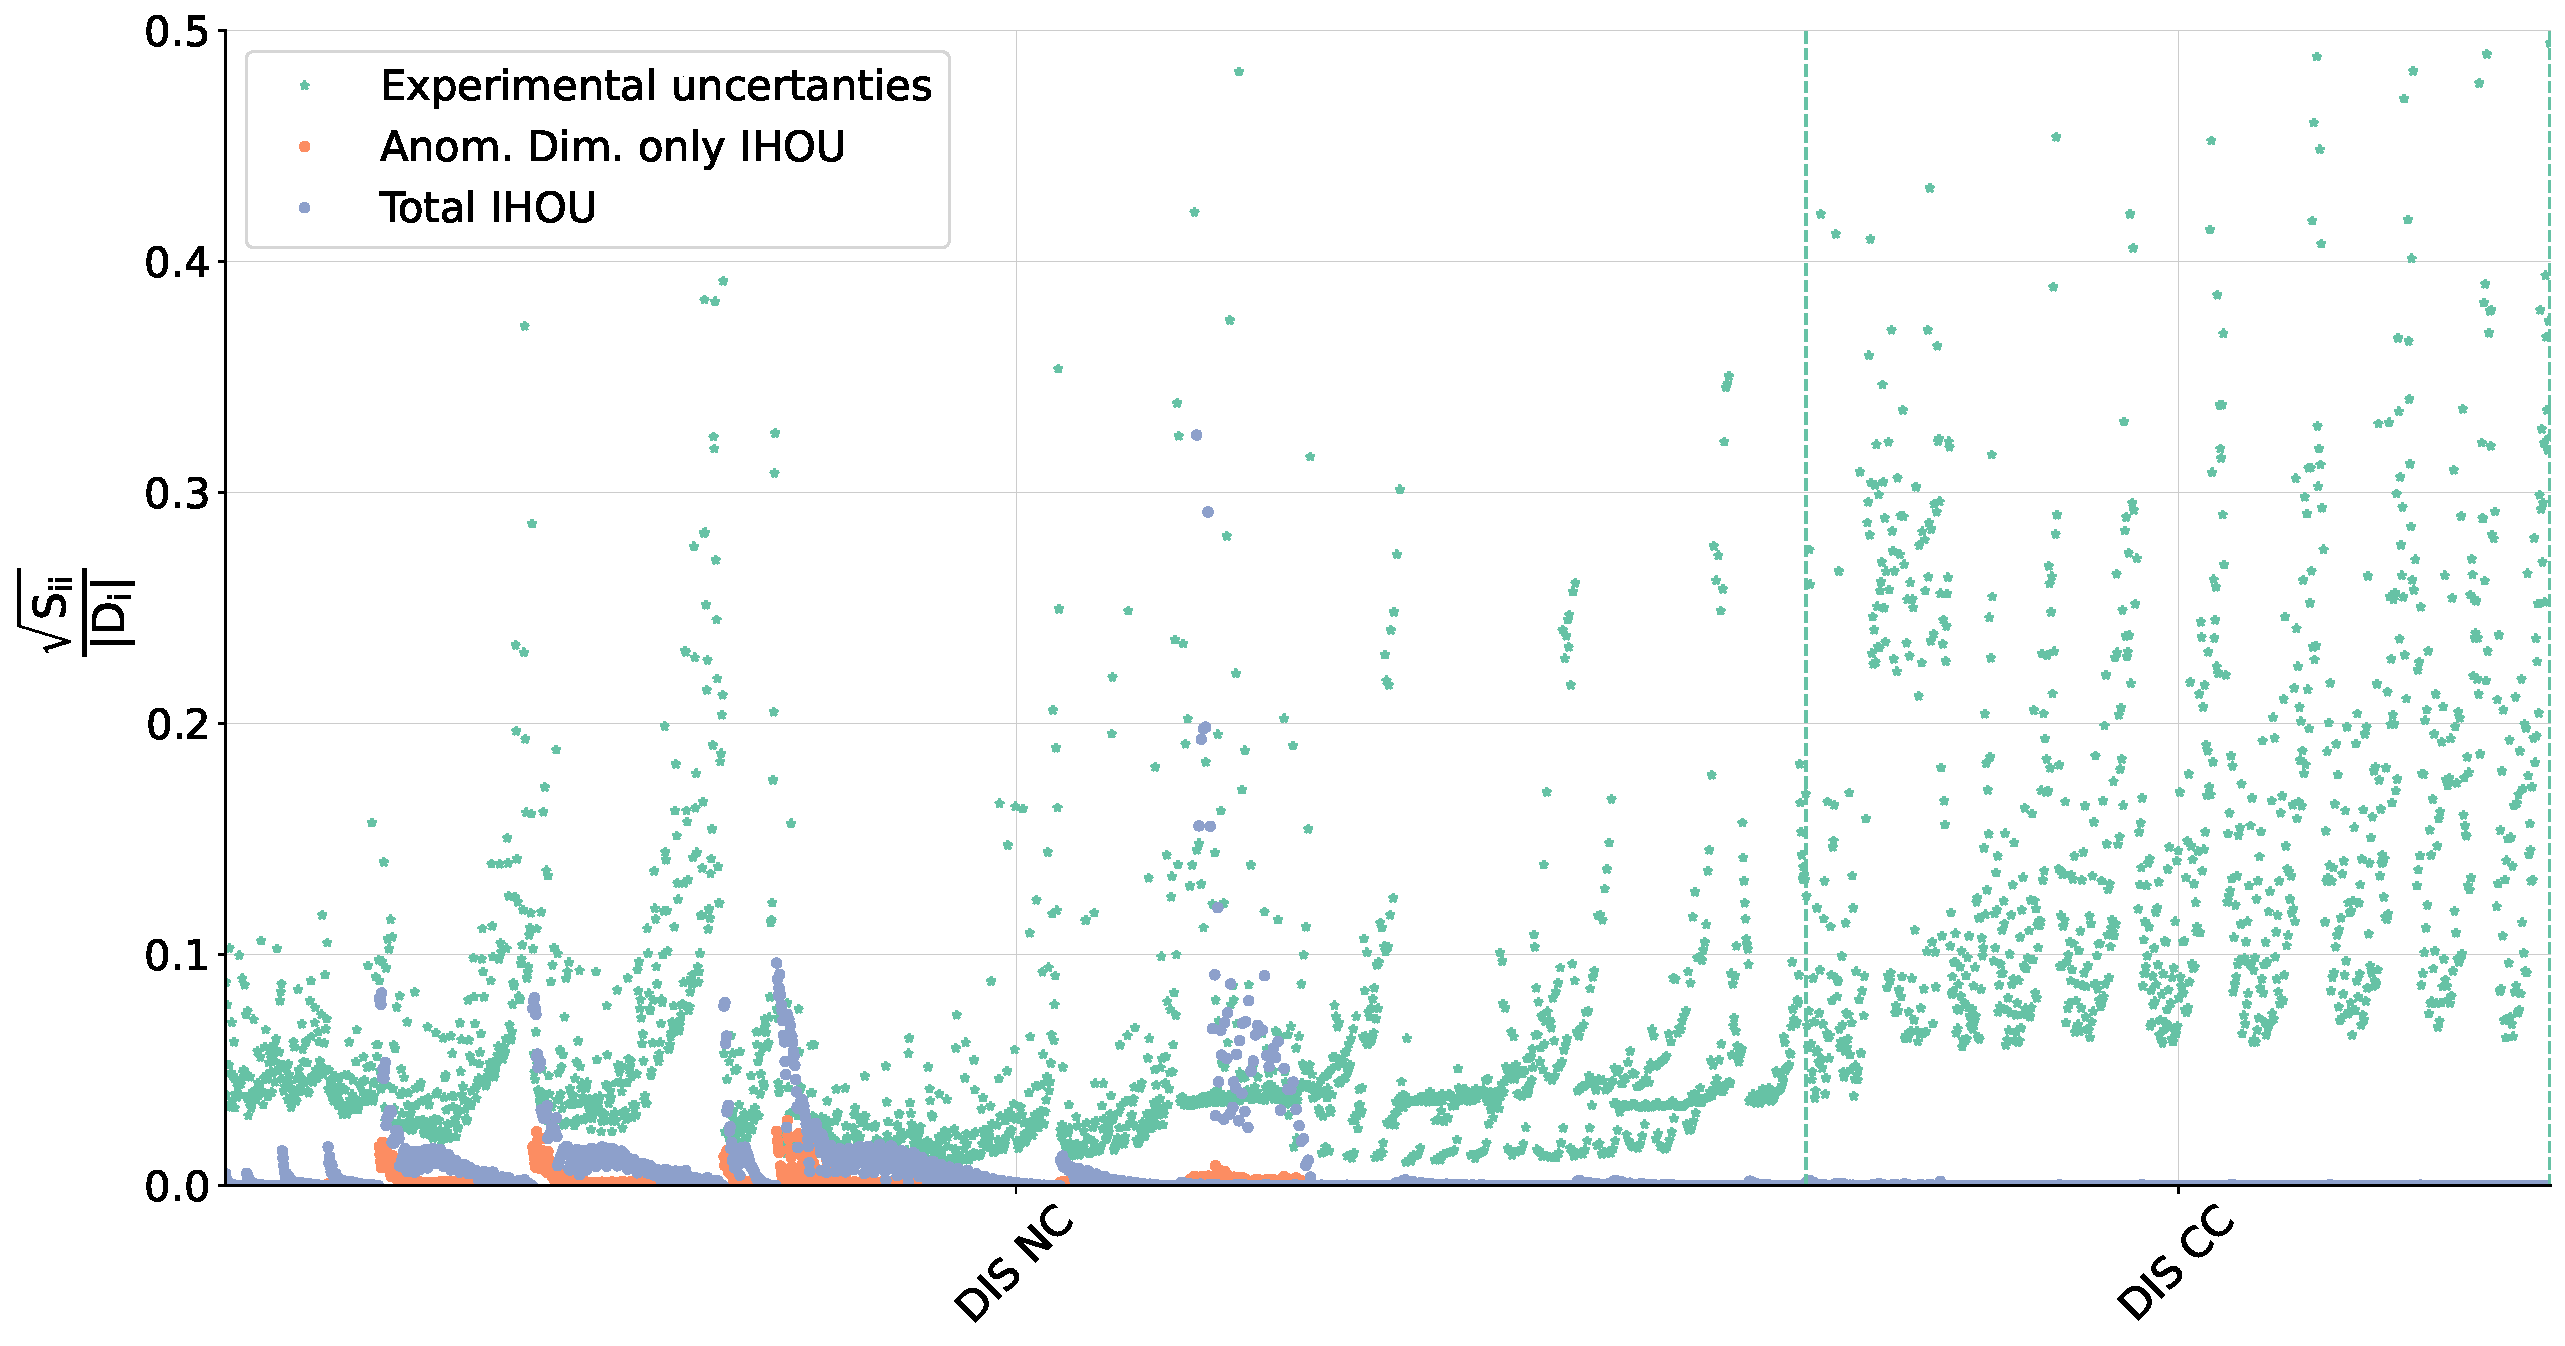
\includegraphics[width=.9\textwidth]{figures/diag_cov_dis_ihou.pdf}
        \caption*{IHOU have a large effect on small-$x$, low-$Q$ DIS data
        }
      \end{figure}
    \end{column}
    \begin{column}{0.49\textwidth}
      \begin{figure}[!t]
        \centering
        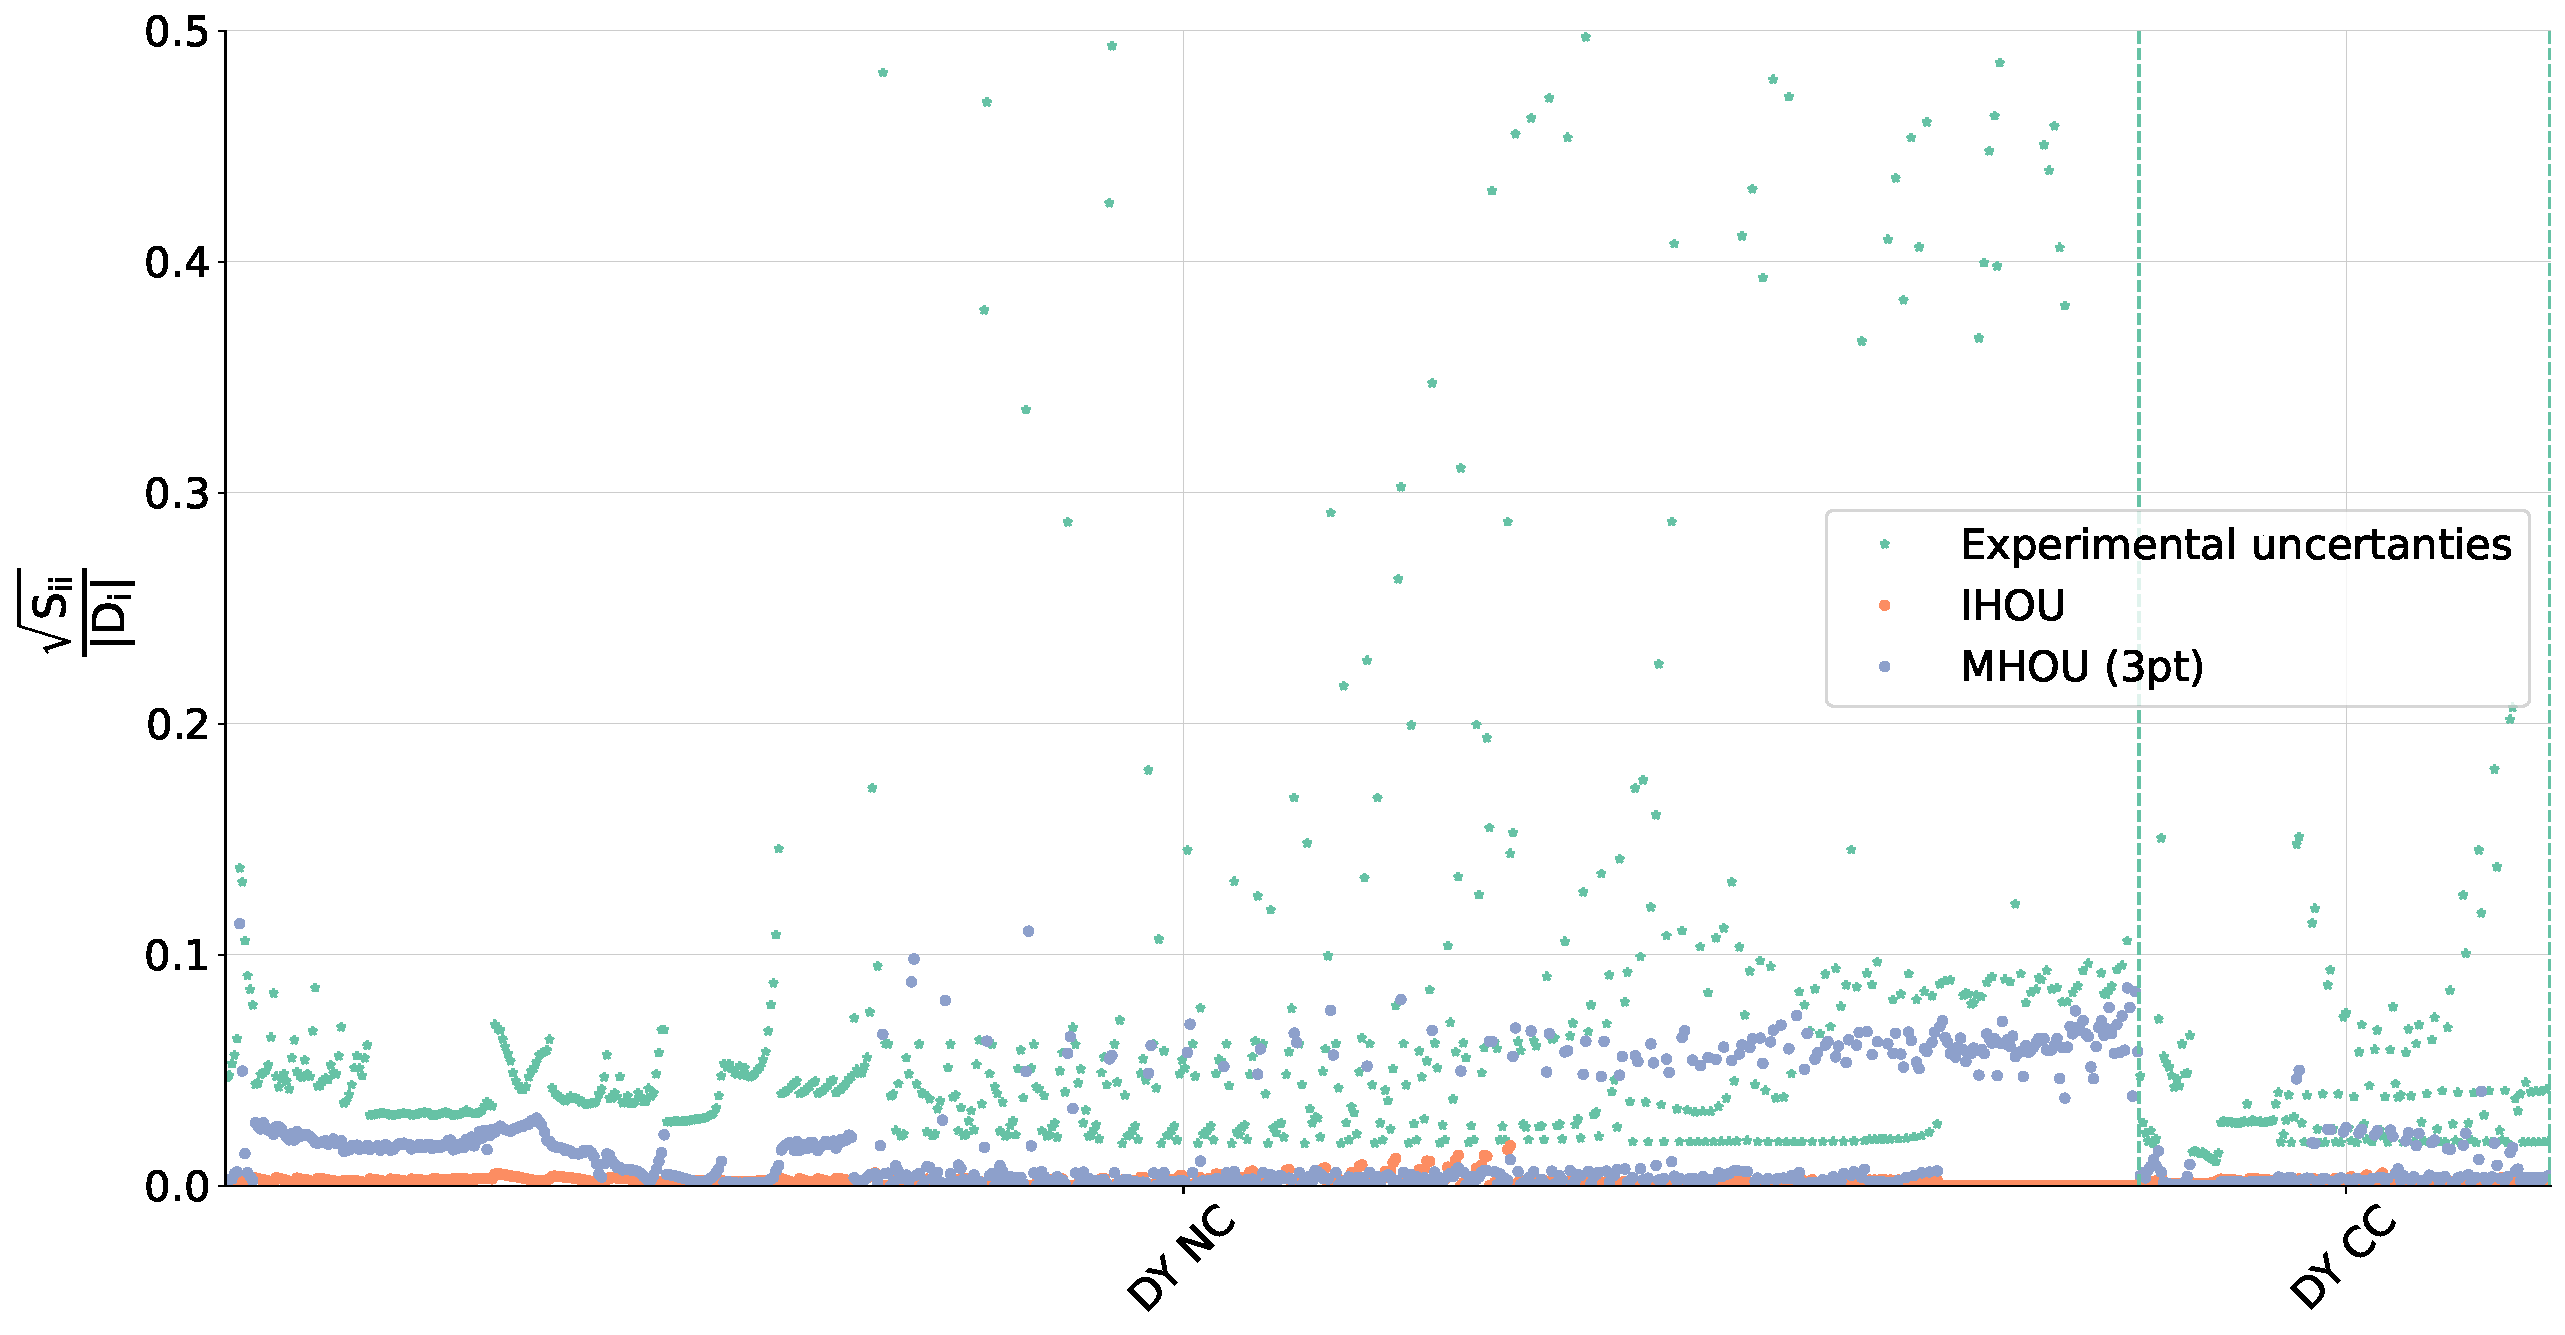
\includegraphics[width=.9\textwidth]{figures/diag_cov_dy_ihou_3pt_mhou.pdf}
        \caption*{NNLO MHOU included where N3LO not available \\
          MHOU can similar magnitude as the experimental uncertainty
        }
      \end{figure}
    \end{column}
  \end{columns}


\end{frame}

% \begin{frame}{Magnitude of theory uncertainties}
% % show that for certain processes th unc is of same size as exp unc.
% \end{frame}

% ============================================================================

\begin{frame}{Impact of MHOUs at N3LO}
  \begin{figure}[!t]
    \centering
    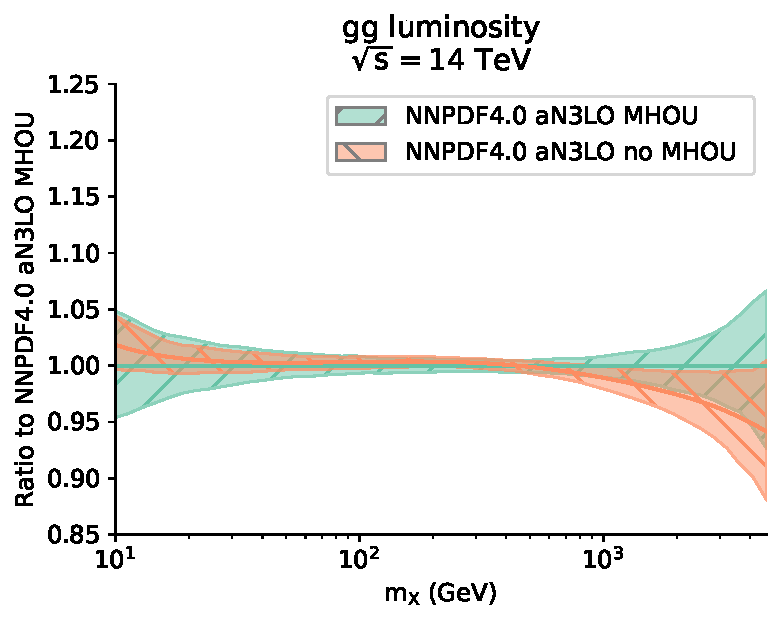
\includegraphics[width=0.45\textwidth]{figures/gg_plot_lumi1d.pdf}
    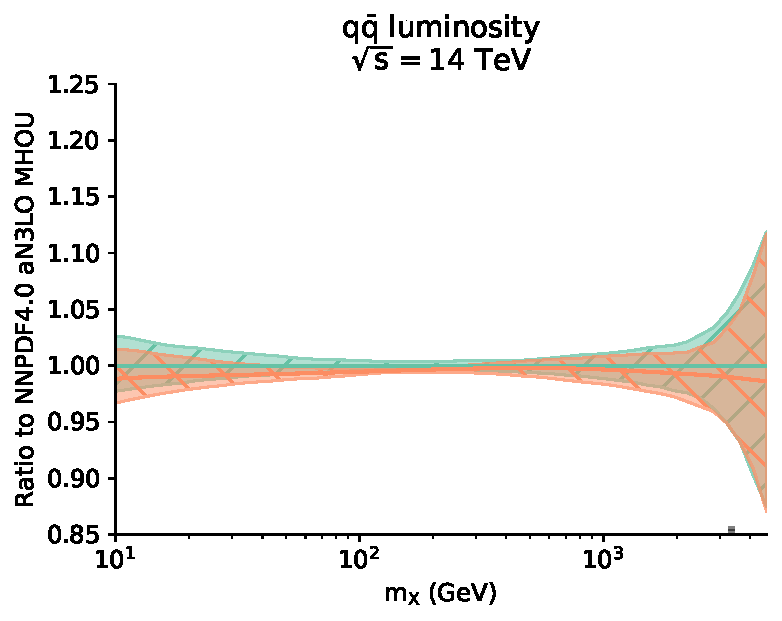
\includegraphics[width=0.45\textwidth]{figures/qqbar_plot_lumi1d.pdf}
  \end{figure}
  \begin{itemize}
    \item Non-negligible impact of MHOUs even at N3LO
    \item[$\Rightarrow$] reason to include exact N3LO calculations for hadronic processes
  \end{itemize}
\end{frame}


% \begin{frame}{Comparison to MSHT20}
%   \begin{figure}[!t]
%     \centering
%     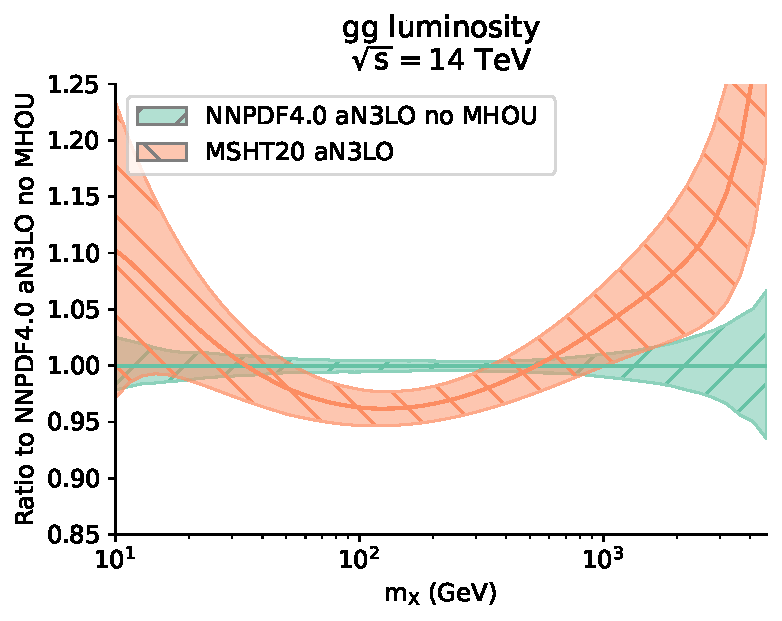
\includegraphics[width=0.45\textwidth]{figures/gg_plot_lumi1d_msht20.pdf}
%     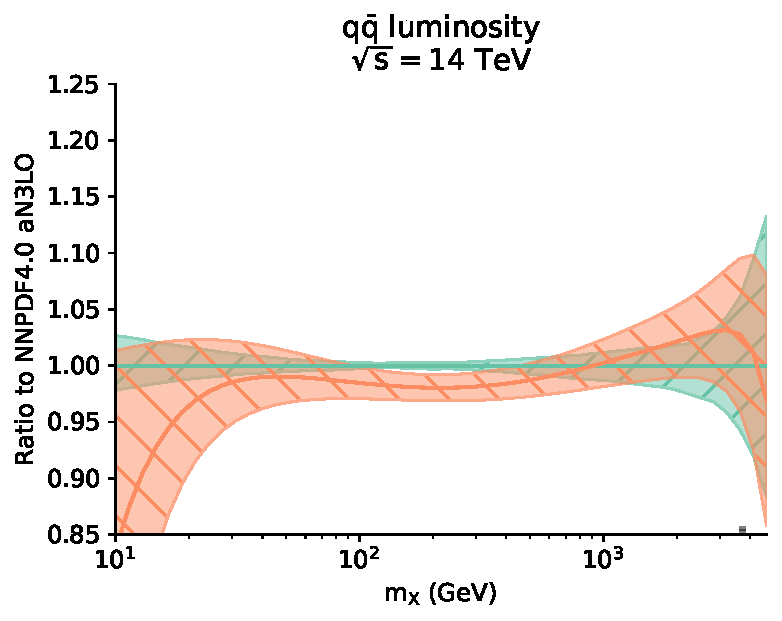
\includegraphics[width=0.45\textwidth]{figures/qqbar_plot_lumi1d_msht20.pdf}
%   \end{figure}
%   \begin{itemize}
%     \item Good agreement with MSHT20 for the quark luminosities
%     \item Also for gluon luminosities, except around the Higgs mass and high-mass
%     \item Similar data but different methodology (including splitting function parametrization)
%   \end{itemize}
% \end{frame}









\end{document}
